\section{Latches und FlipFlops}
\begin{center}
    \begin{minipage}[t]{0.45\linewidth}
        \paragraph{Kombinatorische Schaltung}
        Output hängt von Inputs und Verknüpfungen ab.
    \end{minipage}
    \hfill
    \begin{minipage}[t]{0.45\linewidth}
        \paragraph{Sequentielle Schaltung}
        Enthält Rückkopplungen, Outputs hängen von vorherigen Werten ab.
    \end{minipage}
\end{center}
\hrule
\begin{center}
    \begin{minipage}[t]{0.45\linewidth}
        \paragraph{Latch}
        \emph{(Takt)\underline{zustand}gesteurte} Schaltung $\rightarrow$ Änderungen am Eingang können während der \emph{ganzen aktiven Taktphase} den Output beeinflussen.
    \end{minipage}
    \hfill
    \begin{minipage}[t]{0.45\linewidth}
        \paragraph{FlipFlops}
        \emph{Takt\underline{flanken}gesteuerte} Schaltung $\rightarrow$ Input zum Zeitpunkt der Taktwechsels wird wirksam.
    \end{minipage}
\end{center}
\subsection{Latches}
Alle taktzustandgesteurte Schaltungen sind gegenüber \cemph[burntorange]{Störimpulsen} empfindlich, da bei $\text{T}=1$ jede Änderung übernommen wird.
\subsubsection{SR-Latch}
\begin{center}
    \begin{minipage}[c]{0.4\linewidth}
        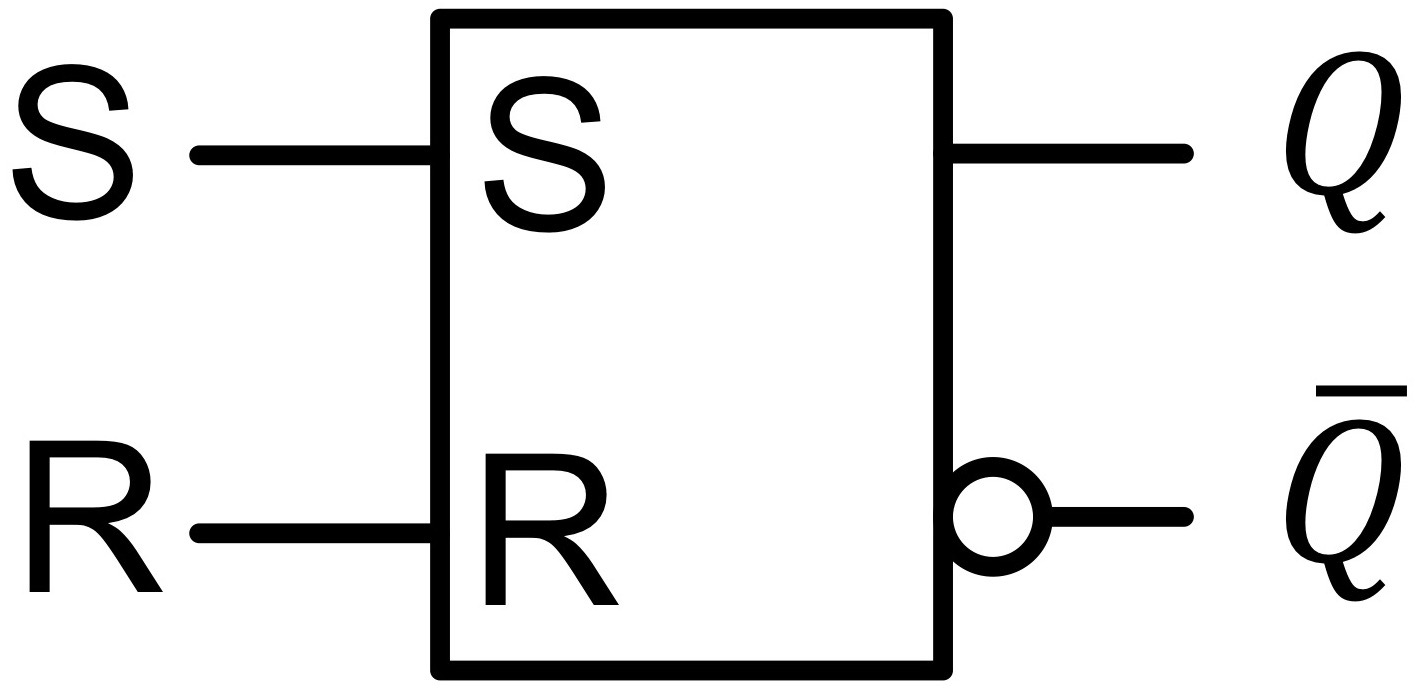
\includegraphics[width = 23mm]{images/sr_latch.jpeg}
    \end{minipage}
    \hfill
    \begin{minipage}[c]{0.55\linewidth}
        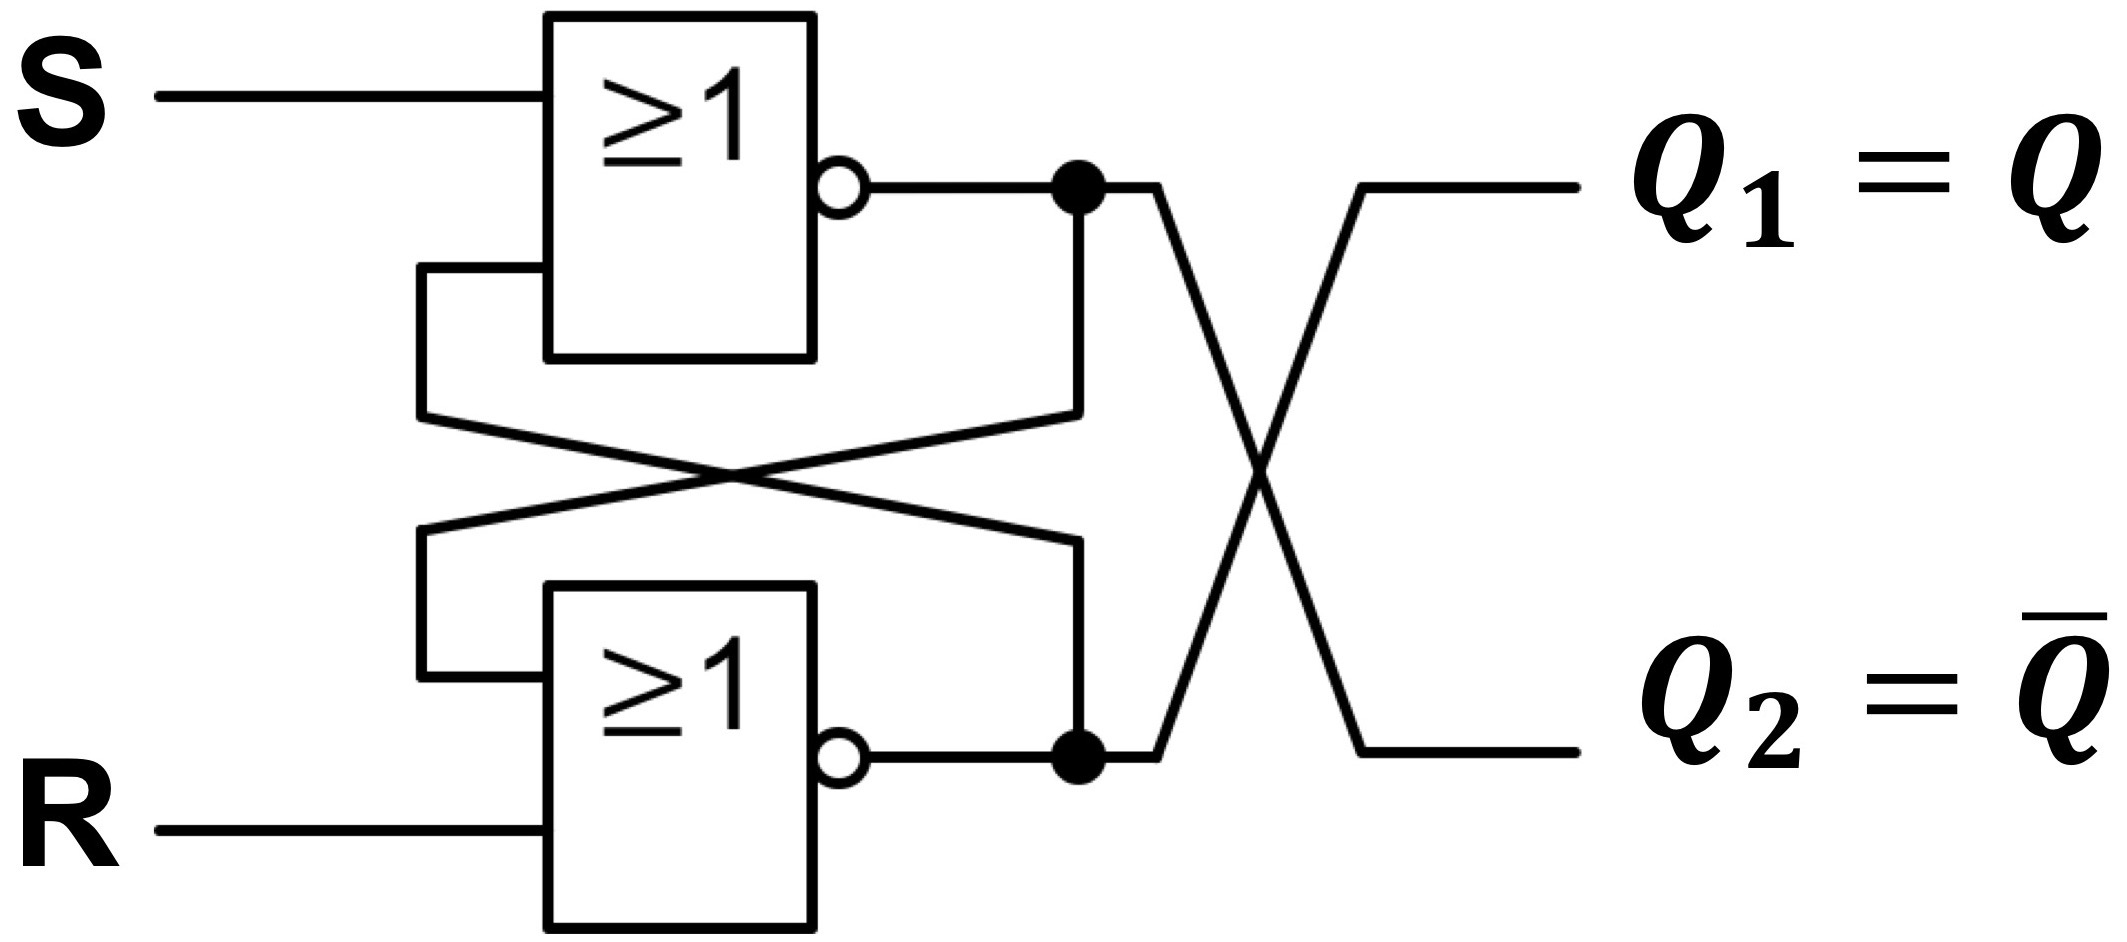
\includegraphics[width = 35mm]{images/sr_latch_cir.jpeg}
    \end{minipage}
\end{center}
\begin{flushleft}
    \begin{tabular}{l l c l}
        \textbf{S} & Set & $\rightarrow$ & setzt $Q$ auf $1$\\
        \textbf{R} & Reset & $\rightarrow$ & setzt $Q$ auf $0$\\
    \end{tabular}
\end{flushleft}
\begin{equation*}
    Q_{n + 1} = S \lor \left(Q_n \land \overline{R}\right)
\end{equation*}
\begin{center}
    \begin{tabular}{c|c c|c l}
        Fall & \textbf{S} & \textbf{R} & $Q_{n + 1}$ & \\
        \cline{1-4}
        1 & $0$ & $0$ & $Q_n$ & speichern\\        
        2 & $0$ & $1$ & $0$ & zurücksetzten\\        
        3 & $1$ & $0$ & $1$ & setzen\\        
        4 & $1$ & $1$ & - & unzulässig\\        
    \end{tabular}
\end{center}
\subsubsection{SRT-Latch}
\begin{center}
    \begin{minipage}[c]{0.4\linewidth}
        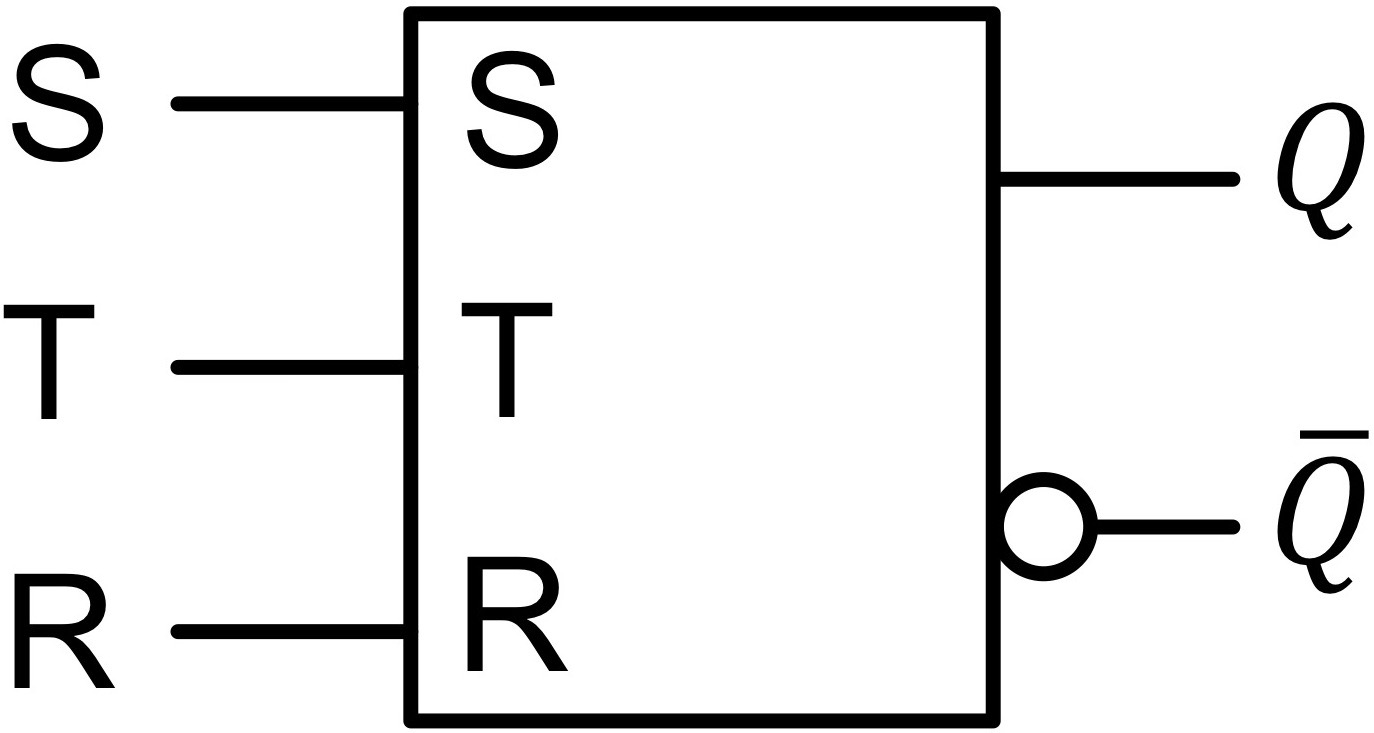
\includegraphics[width = 23mm]{images/srt_latch.jpeg}
    \end{minipage}
    \hfill
    \begin{minipage}[c]{0.55\linewidth}
        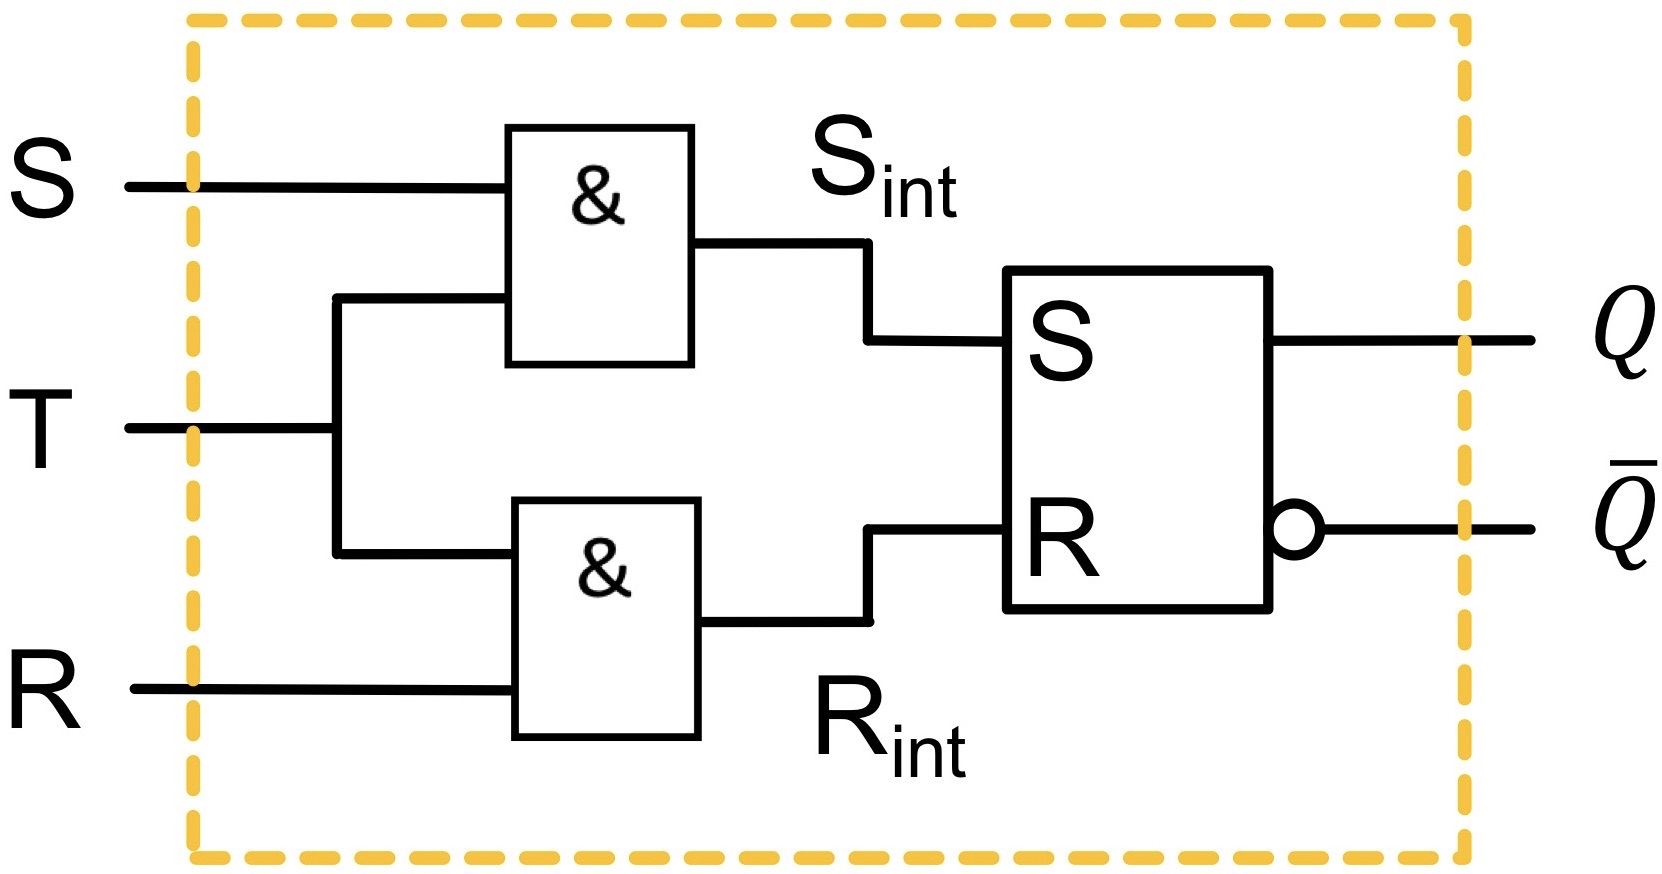
\includegraphics[width = 35mm]{images/srt_latch_cir.jpeg}
    \end{minipage}
\end{center}
\begin{flushleft}
    \begin{tabular}{c c c c c l}
        T & & $\text{S}_{\text{int}}$ & $\text{R}_{\text{int}}$ & &\\
        $0$ & $\rightarrow$ & $0$ & $0$ & $\rightarrow$ & Datenspeicherung\\
        $1$ & $\rightarrow$ & S & R & $\rightarrow$ & Normales SR-Latch\\
    \end{tabular}
\end{flushleft}
Änderungen werden nur übernommen, wenn T/CLK aktiv ist.

\subsubsection{D-Latch}
\begin{center}
    \begin{minipage}[c]{0.4\linewidth}
        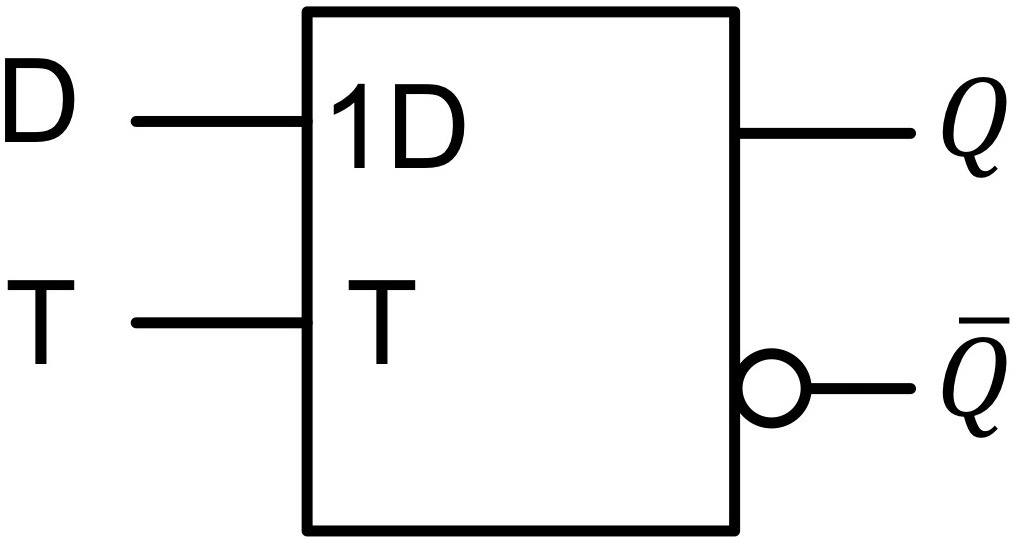
\includegraphics[width = 23mm]{images/d_latch.jpeg}
    \end{minipage}
    \hfill
    \begin{minipage}[c]{0.55\linewidth}
        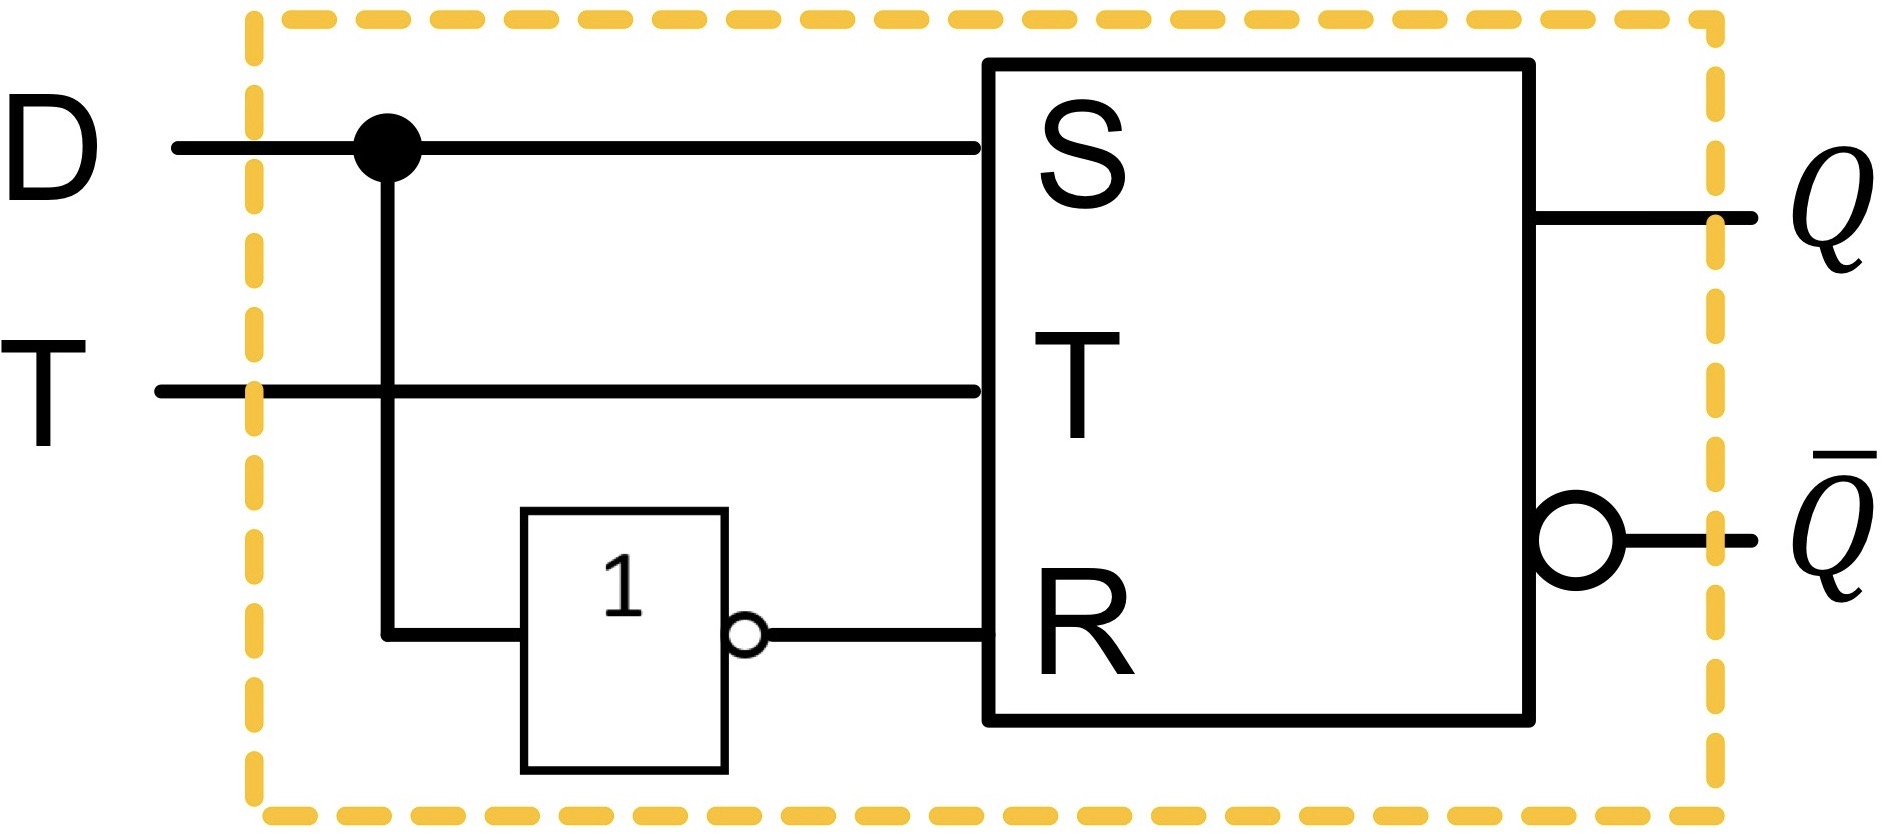
\includegraphics[width = 35mm]{images/d_latch_cir.jpeg}
    \end{minipage}
\end{center}
Bauelement, das Daten für die Periodendauer eines Taktes speichern kann.
\begin{equation*}
    Q_{n + 1} = \left(Q_n \land \overline{\text{T}}\right) \lor \left(\text{D} \land \text{T}\right)
\end{equation*}
\begin{flushleft}
    \begin{tabular}{c c c l}
        T & $Q_{n + 1}$ & & \\
        $0$ & $Q_n$ & $\rightarrow$ & alter Ausgang gespeichert\\
        $1$ & D & $\rightarrow$ & Input übernommen\\
    \end{tabular}
\end{flushleft}
\begin{center}
    \begin{tikzpicture}
        \begin{pgfonlayer}{bg}
            \fill[red!30] (0,0) rectangle (1, -0.5);
            \fill[darkgreen!30] (1,0) rectangle (2, -0.5);
        \end{pgfonlayer}
        \draw[thick] (-1, -0.5) -- (0, -0.5) -- (0,0) -- (1, 0) -- (1, -0.5) -- (2, -0.5) -- (2,0) -- (3, 0);
        \begin{pgfonlayer}{tl1}
            \node[draw = red] (t1) at (-1, 0.5) {\small D-Latch transparent};
            \node[draw = darkgreen] (t2) at (2.5, 0.5) {\small letzter Zustand gespeichert};
        \end{pgfonlayer}
        \draw[red] (t1) -- (0.5, 0);
        \draw[darkgreen] (t2) -- (1.5, 0);
    \end{tikzpicture}
\end{center}

\subsection{FlipFlops}
\begin{center}
    \begin{minipage}{0.45\linewidth}
        \begin{center}
            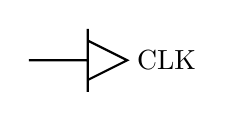
\begin{tikzpicture}
                \draw[thick] (-0.75, 0) -- (0,0)
                    (0,0.4) -- (0,-0.4)
                    (0,0.25) -- (0.5,0) -- (0,-0.25);
                \node[] at (1, 0) {CLK};
            \end{tikzpicture}
        \end{center}
        Input beim Übergang von \emph{$0 \rightarrow 1$} von CLK wirksam.
        \begin{center}
            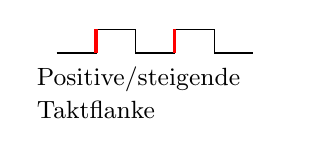
\begin{tikzpicture}
                \draw (0,0) -- (0.5, 0) -- (0.5, 0.3) -- (1, 0.3) -- (1, 0) -- (1.5, 0) -- (1.5, 0.3) -- (2, 0.3) -- (2, 0) -- (2.5, 0);
                \draw[very thick, red] (0.5, 0) -- (0.5, 0.3) (1.5, 0) -- (1.5, 0.3);
                \node[text width = 30mm] at (1.25, -0.5) {\small Positive/steigende Taktflanke};
            \end{tikzpicture}
        \end{center}
    \end{minipage}
    \hfill
    \begin{minipage}{0.45\linewidth}
        \begin{center}
            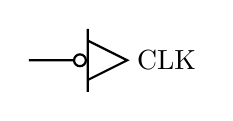
\begin{tikzpicture}
                \draw[thick] (-0.75, 0) -- (0,0)
                    (0,0.4) -- (0,-0.4)
                    (0,0.25) -- (0.5,0) -- (0,-0.25);
                \draw[thick, fill = white] (-0.1,0) circle [radius = 0.75mm];
                \node[] at (1, 0) {CLK};
            \end{tikzpicture}
        \end{center}
        Input beim Übergang von \emph{$1 \rightarrow 0$} von CLK wirksam.
        \begin{center}
            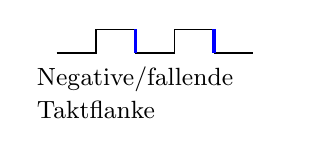
\begin{tikzpicture}
                \draw (0,0) -- (0.5, 0) -- (0.5, 0.3) -- (1, 0.3) -- (1, 0) -- (1.5, 0) -- (1.5, 0.3) -- (2, 0.3) -- (2, 0) -- (2.5, 0);
                \draw[very thick, blue] (1, 0.3) -- (1, 0) (2, 0.3) -- (2, 0);
                \node[text width = 30mm] at (1.25, -0.5) {\small Negative/fallende Taktflanke};
            \end{tikzpicture}
        \end{center}
    \end{minipage}
\end{center}
\subsubsection{D-FlipFlop}
\begin{center}
    \begin{minipage}[c]{0.4\linewidth}
        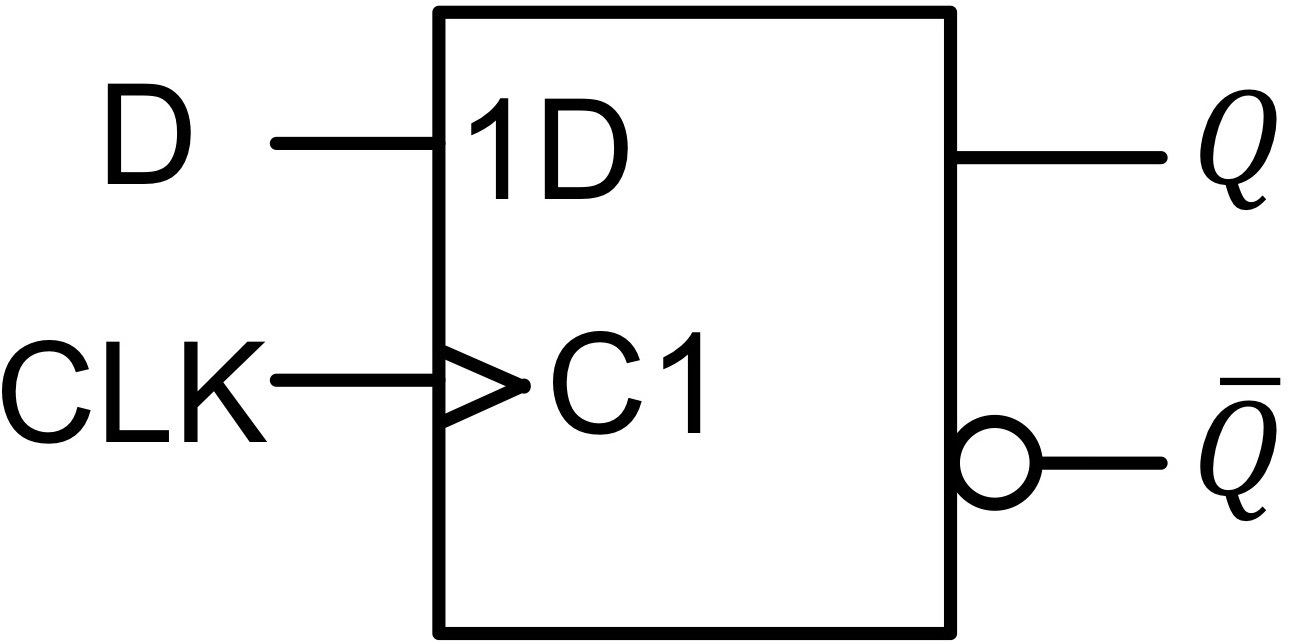
\includegraphics[width = 23mm]{images/d_ff.jpeg}
    \end{minipage}
    \hfill
    \begin{minipage}[c]{0.55\linewidth}
        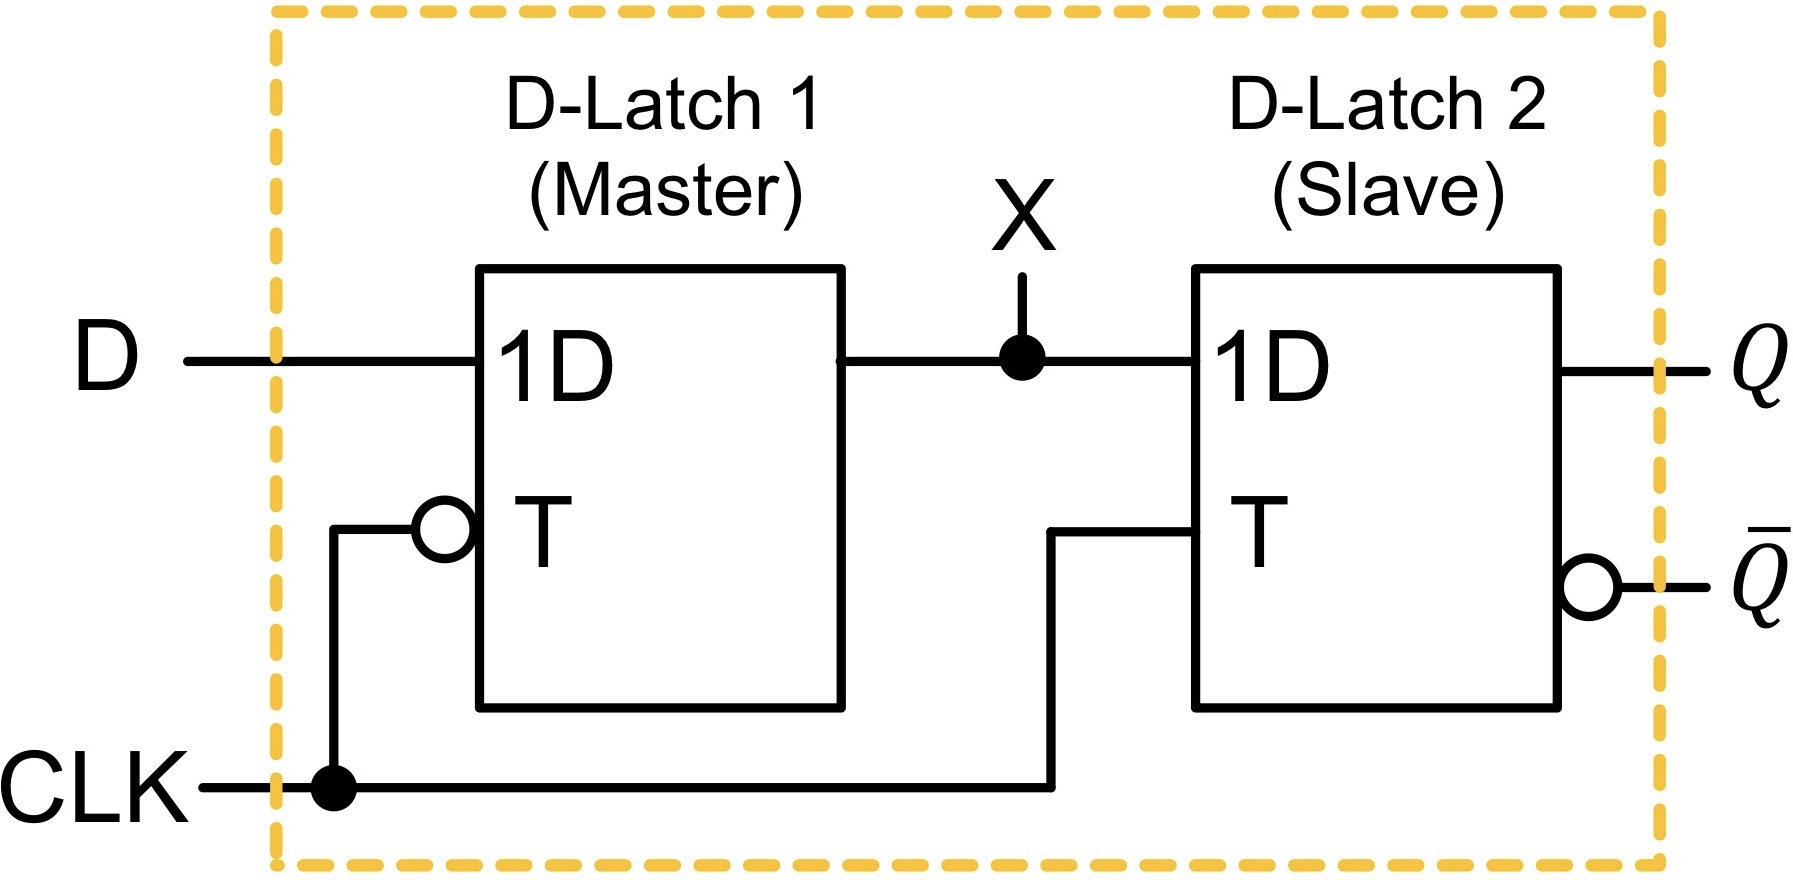
\includegraphics[width = 35mm]{images/d_ff_cir.jpeg}
    \end{minipage}
\end{center}
\begin{equation*}
    Q_{n + 1} = \text{D} \quad \text{wenn} \quad \text{CLK}~0\rightarrow 1 
\end{equation*}
\begin{flushleft}
    \begin{tabular}{l l l}
        Master & low-active & $\text{CLK} = 0$\\
        Slave & high-active & $\text{CLK} = 1$\\
    \end{tabular}
\end{flushleft}
\subsubsection{SR-FlipFlop}
\begin{center}
    \begin{minipage}[c]{0.4\linewidth}
        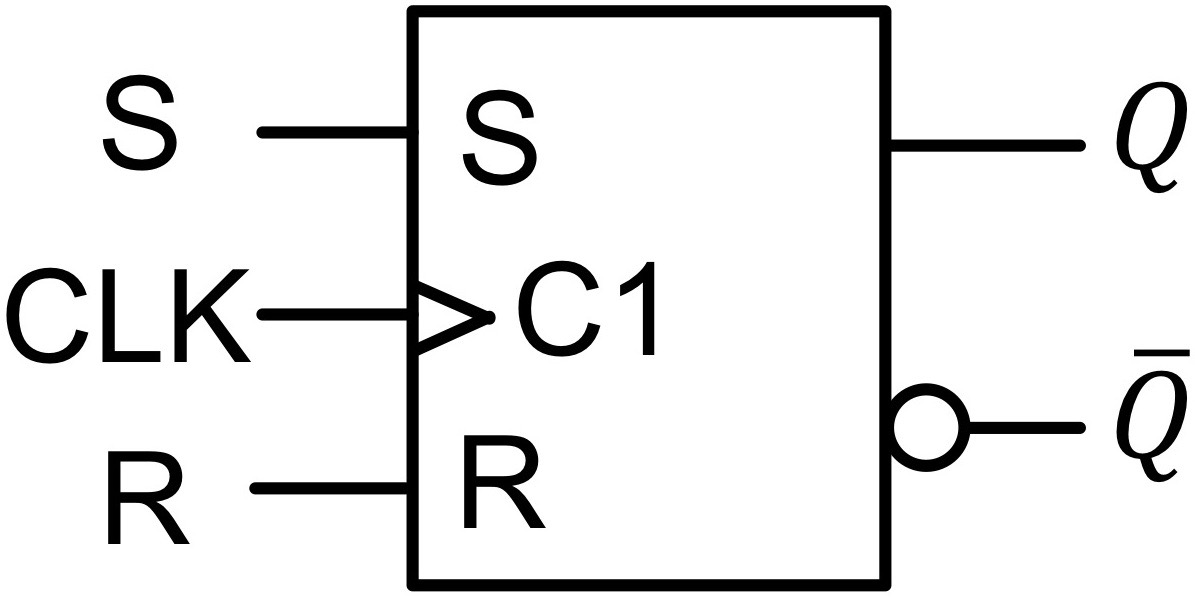
\includegraphics[width = 23mm]{images/srt_ff.jpeg}
    \end{minipage}
    \hfill
    \begin{minipage}[c]{0.55\linewidth}
        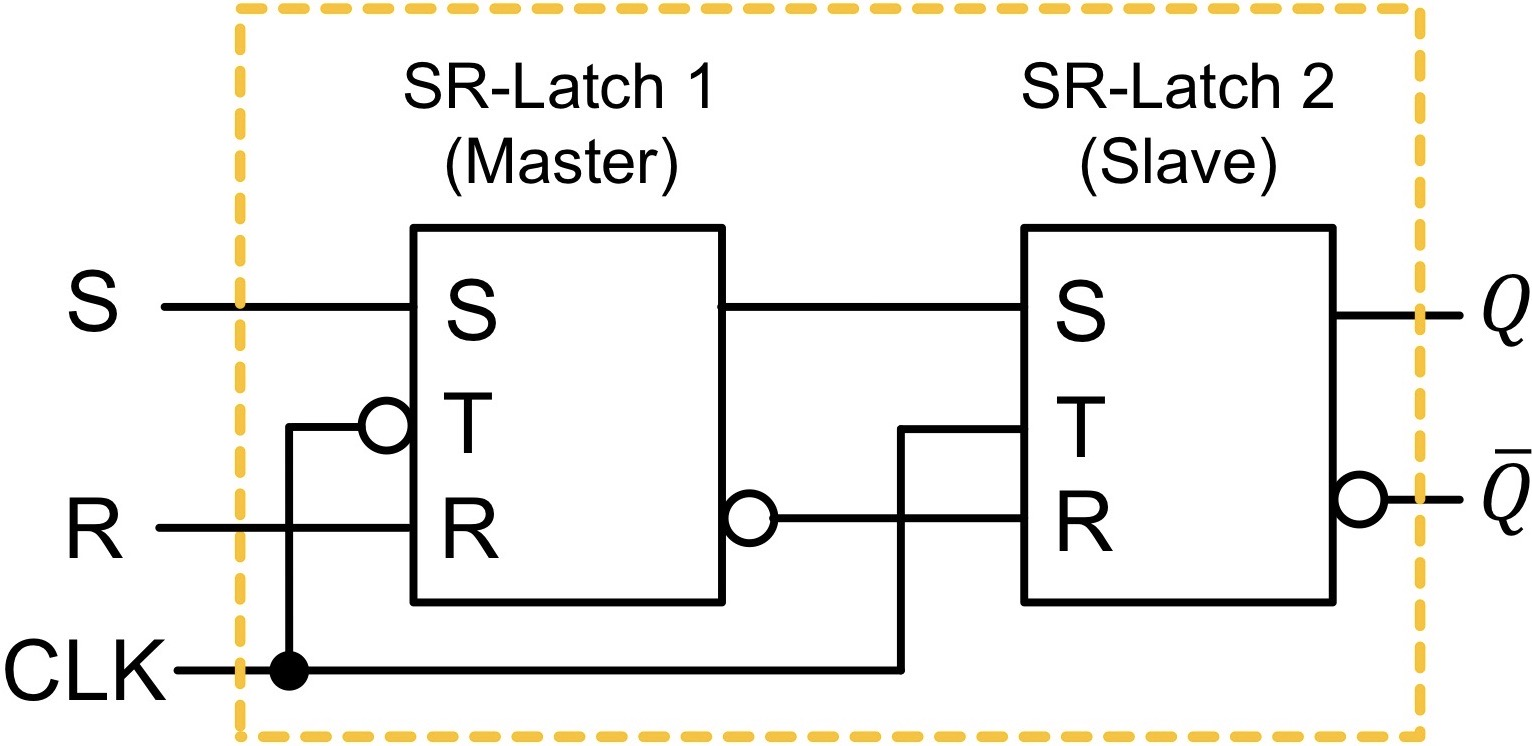
\includegraphics[width = 35mm]{images/srt_ff_cir.jpeg}
    \end{minipage}
\end{center}
\begin{equation*}
    Q_{n + 1} = \text{S} \lor \left(\overline{\text{R}} \land Q_n\right) \quad \text{wenn} \quad \text{CLK}~0\rightarrow 1 
\end{equation*}
\subsubsection{JK-FlipFlop}
\begin{center}
    \begin{minipage}[c]{0.4\linewidth}
        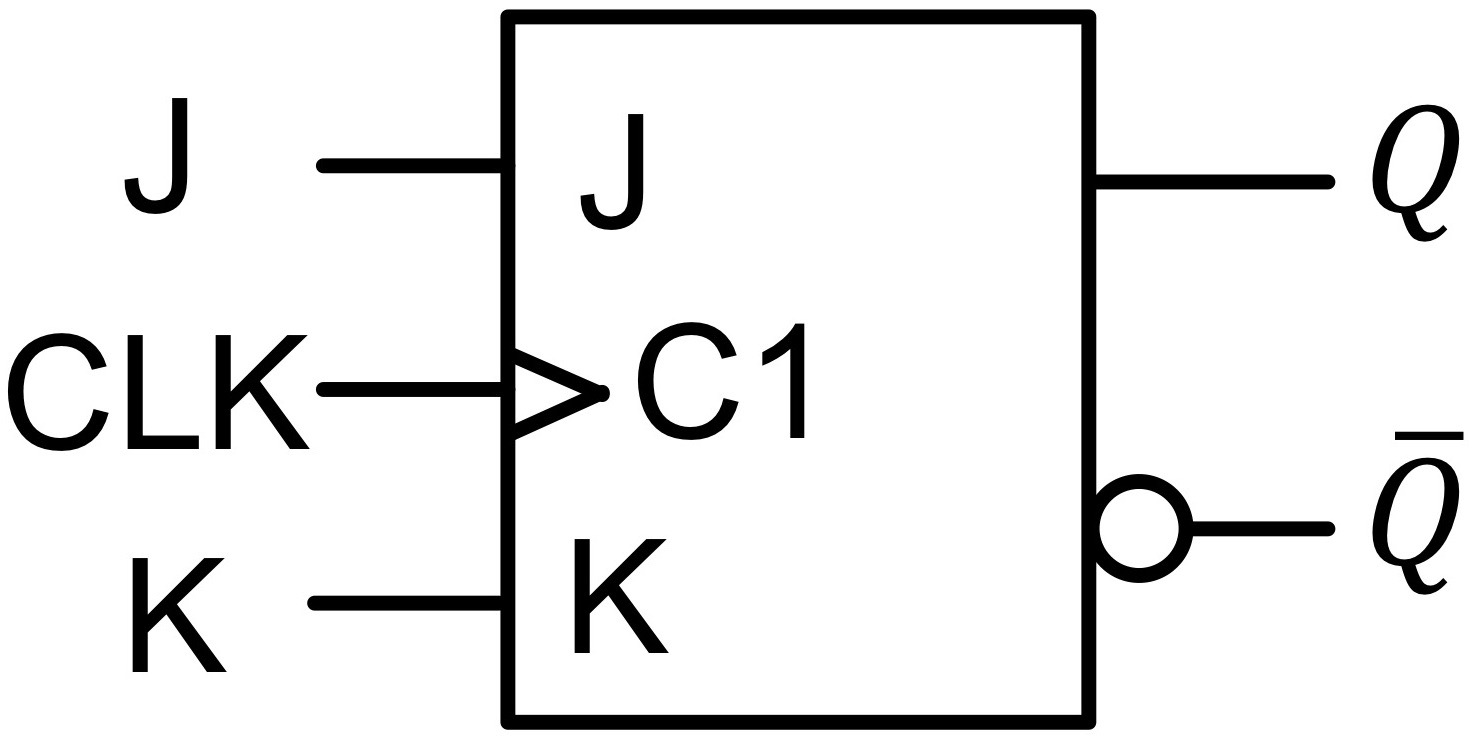
\includegraphics[width = 23mm]{images/jk_ff.jpeg}
    \end{minipage}
    \hfill
    \begin{minipage}[c]{0.55\linewidth}
        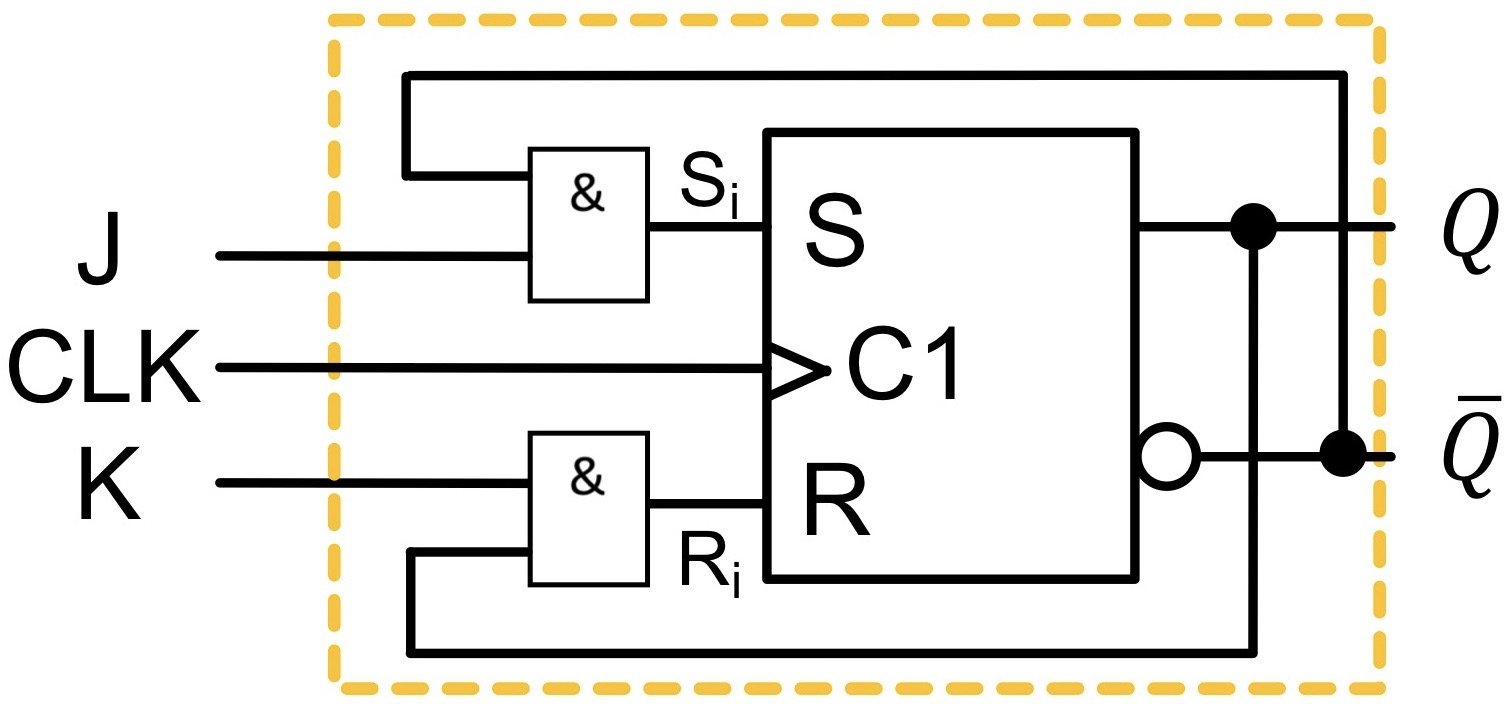
\includegraphics[width = 35mm]{images/jk_ff_cir.jpeg}
    \end{minipage}
\end{center}
\begin{equation*}
    Q_{n + 1} = \left(J \land \overline{Q_n}\right) \lor \left(\overline{K} \land Q_n\right) \quad \text{wenn} \quad \text{CLK}~0\rightarrow 1 
\end{equation*}
\begin{center}
    \begin{tabular}{c|c c|c c l}
        Fall & \textbf{J} & \textbf{K} & $Q_{n + 1}$ & $Q_{n + 1}$ & \\
        \cline{1-5}
        1 & $0$ & $0$ & $Q_{1n}$ & $Q_{2n}$ & speichern\\        
        2 & $0$ & $1$ & $0$ & $1$ & zurücksetzten\\        
        3 & $1$ & $0$ & $1$ & $0$ & setzen\\        
        4 & $1$ & $1$ & $\overline{Q_{1n}}$ & $\overline{Q_{2n}}$ & wechseln\\        
    \end{tabular}
\end{center}
Bei $\text{J}=\text{K}=1$ wechselt Output. (toggel).
\subsubsection{T-FlipFlop}
\begin{center}
    \begin{minipage}[t]{0.45\linewidth}
        \paragraph{V1} Ausgang wechselt bei jeder aktiven Taktflanke.
        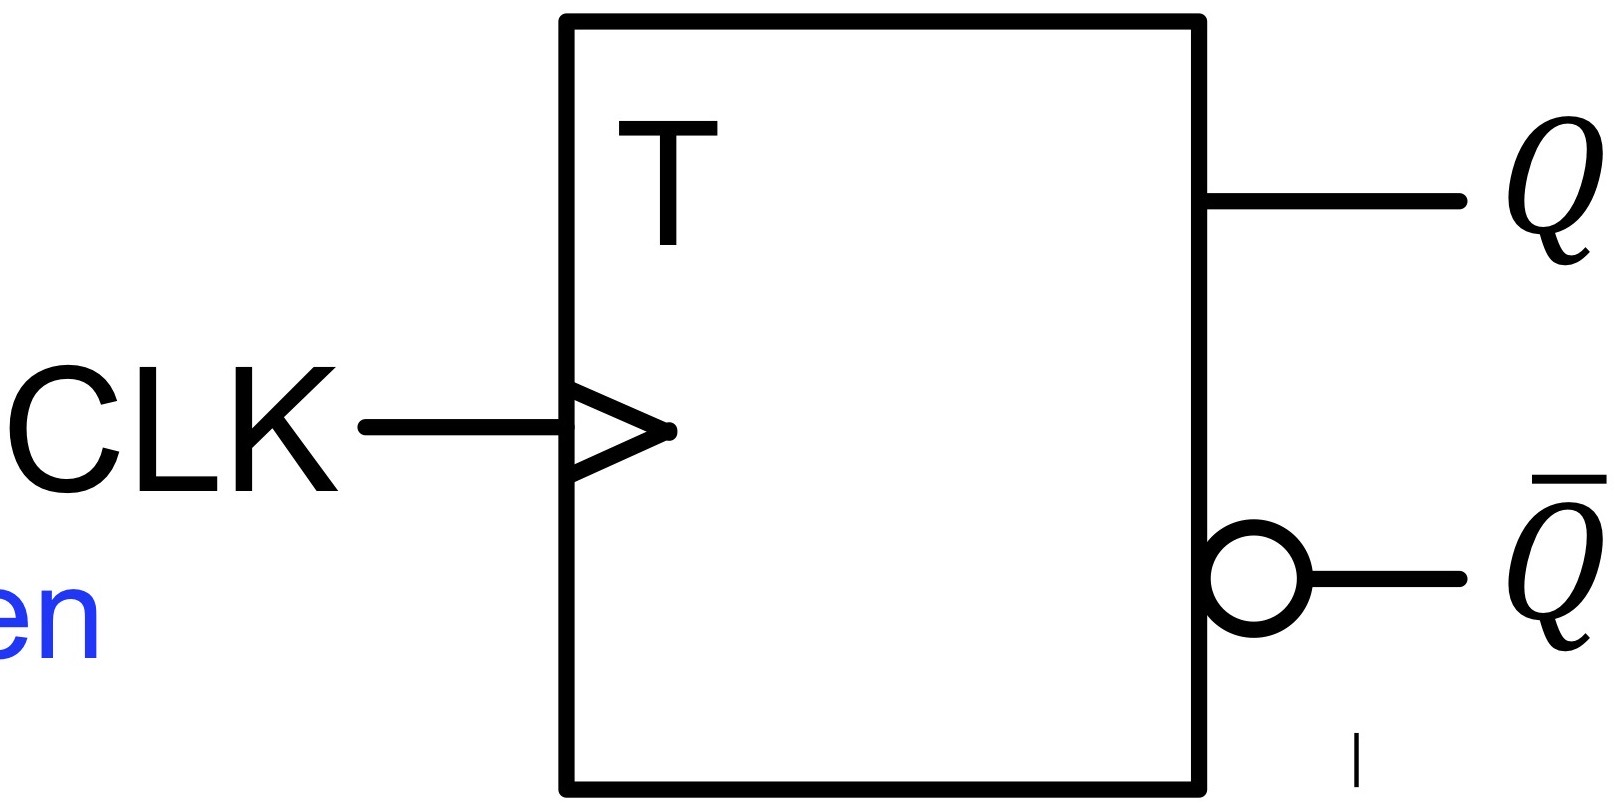
\includegraphics[height = 10mm]{images/t_ff_1.jpeg}
        \begin{align*}
            &Q_{n + 1} = \overline{Q_n}\\
            &\text{wenn CLK}~0\rightarrow 1 
        \end{align*}
    \end{minipage}
    \hfill
    \begin{minipage}[t]{0.45\linewidth}
        \paragraph{V2} Ausgang wechselt bei aktiver Taktflanke nur wenn \emph{$T = 1$}.
        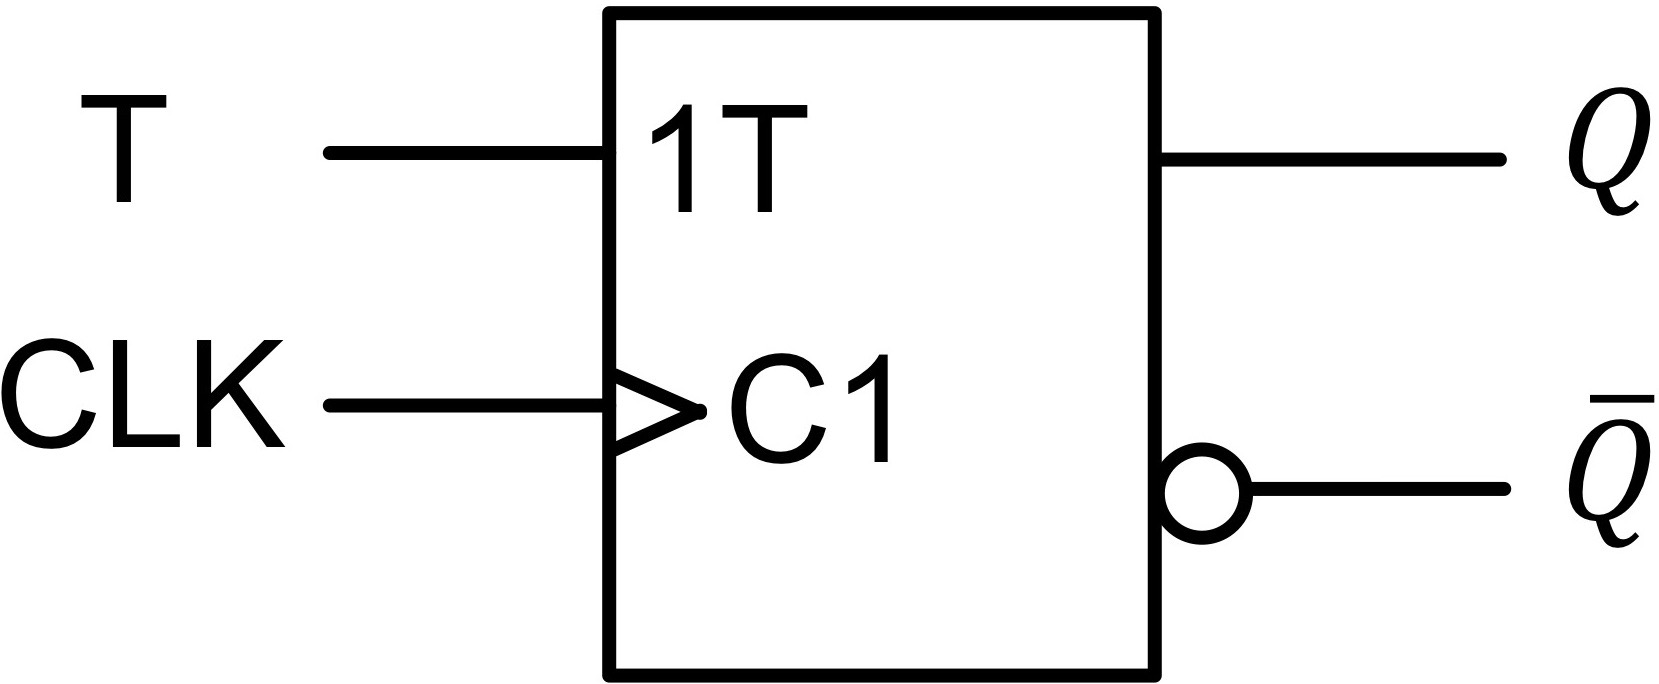
\includegraphics[height = 10mm]{images/t_ff_2.jpeg}
        \begin{align*}
            &Q_{n + 1} = \overline{Q_n}\\
            &\text{wenn CLK}~0\rightarrow 1 \land T = 1
        \end{align*}
    \end{minipage}
\end{center}
\begin{center}
    \begin{minipage}[t]{0.3\linewidth}
        \begin{flushleft}
            BS V1
        \end{flushleft}
        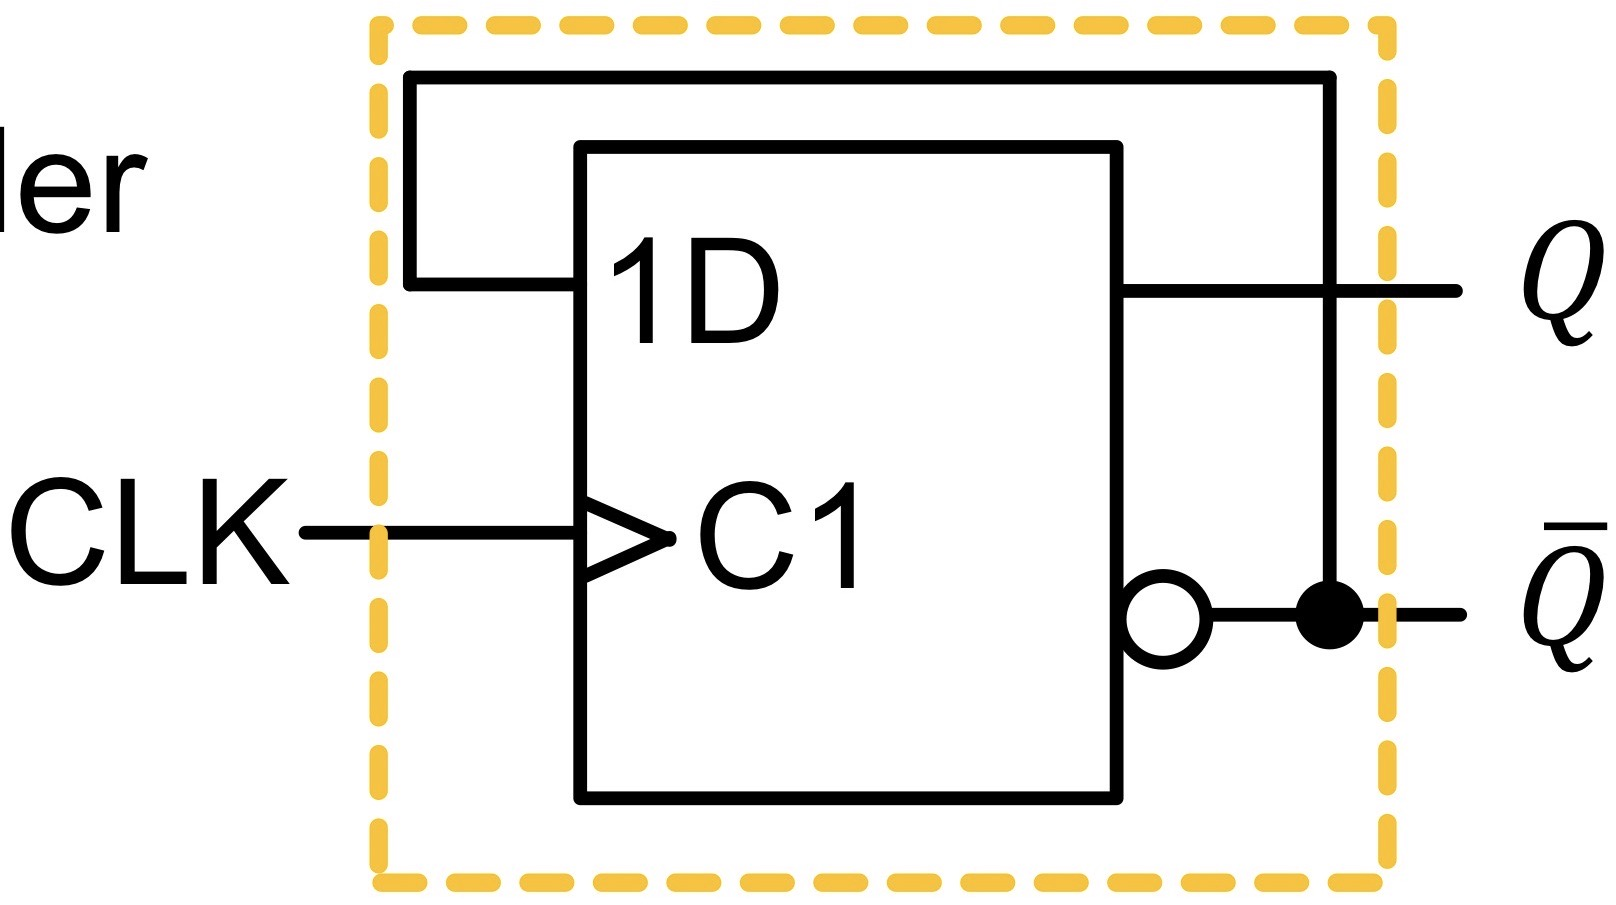
\includegraphics[width = 20mm]{images/t_ff_cir_11.jpeg}
    \end{minipage}
    \hfill\vline\hfill
    \begin{minipage}[t]{0.3\linewidth}
        \begin{flushleft}
            BS V1
        \end{flushleft}
        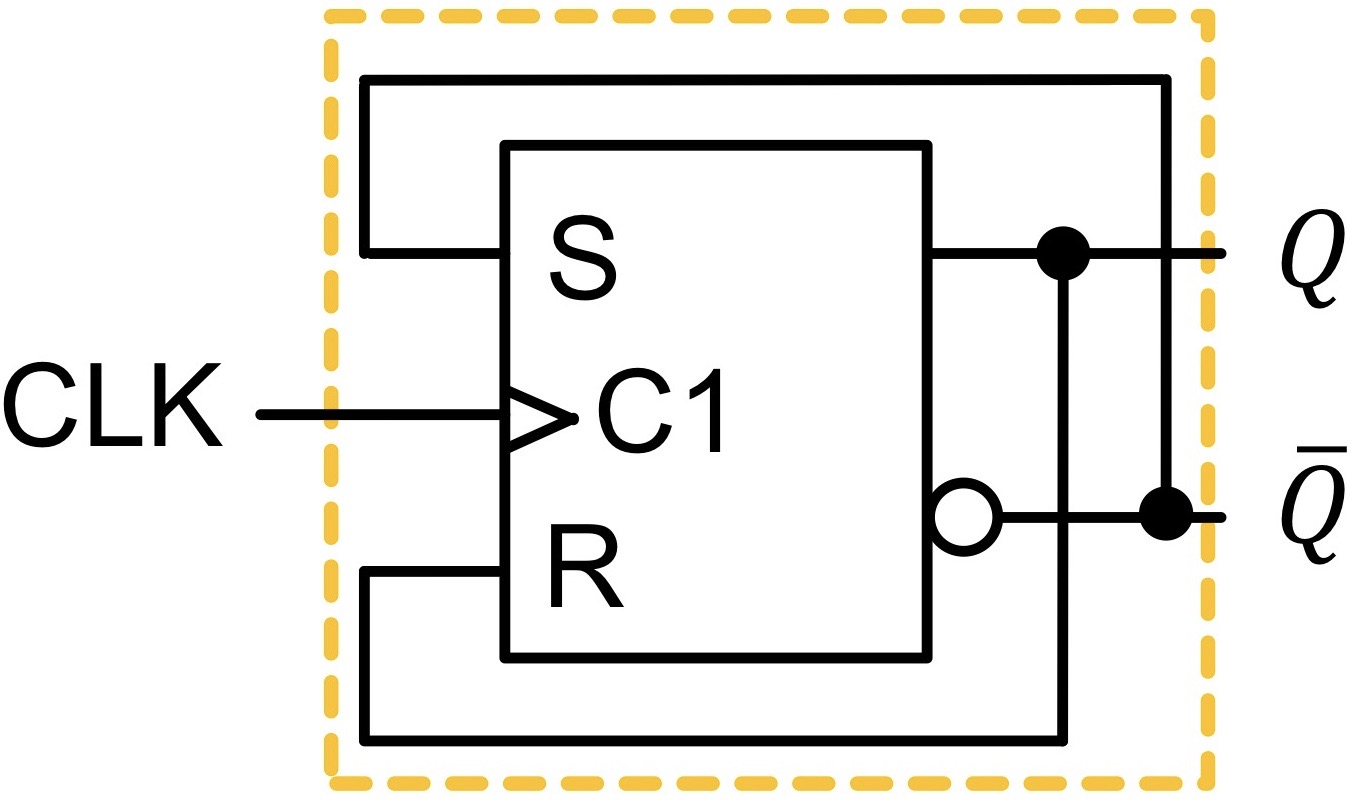
\includegraphics[width = 20mm]{images/t_ff_cir_12.jpeg}
    \end{minipage}
    \hfill\vline\hfill
    \begin{minipage}[t]{0.3\linewidth}
        \begin{flushleft}
            BS V2
        \end{flushleft}
        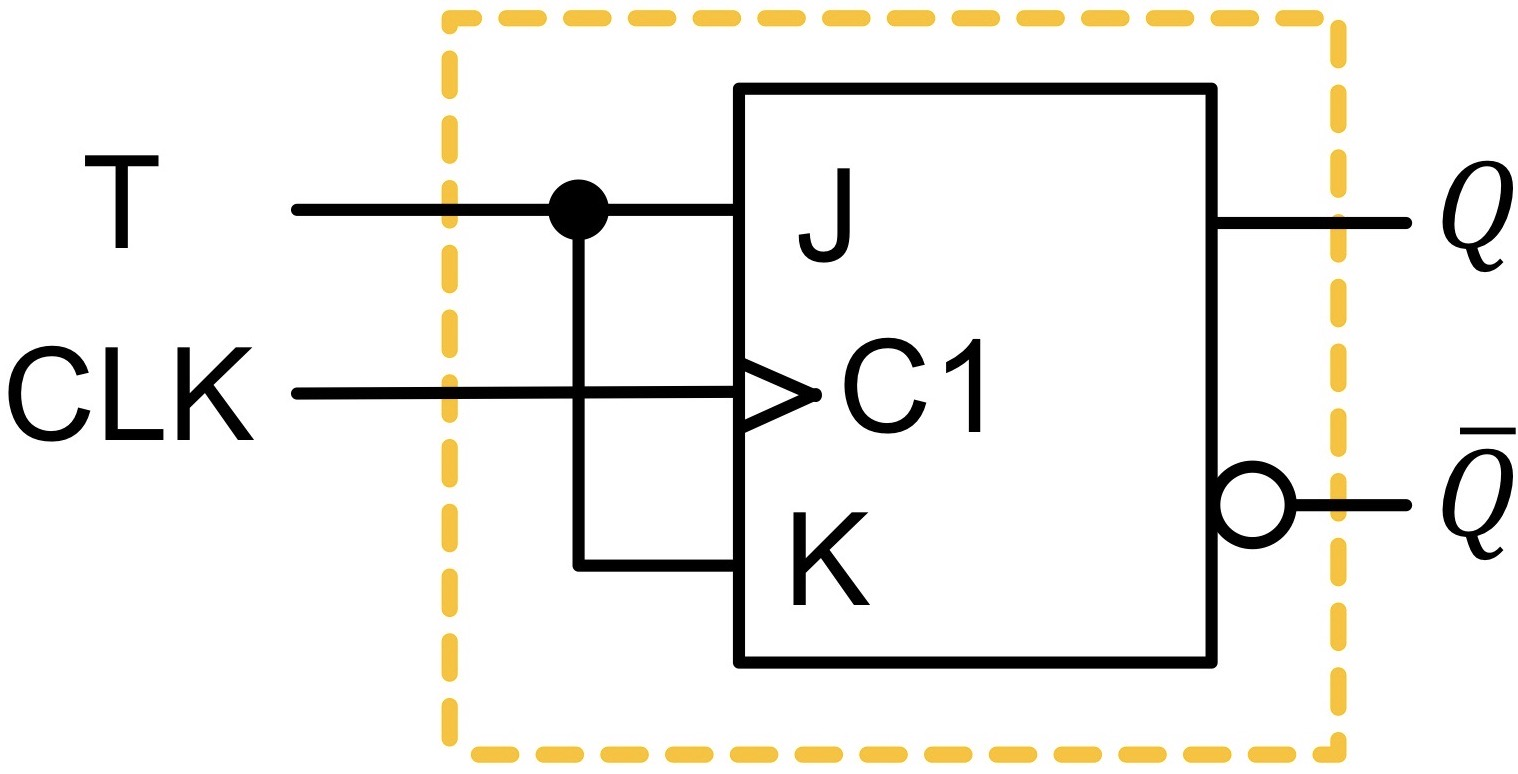
\includegraphics[width = 20mm]{images/t_ff_cir_21.jpeg}
    \end{minipage}
\end{center}

\subsubsection{D-FlipFlop in CMOS-Technik}
\paragraph{Transmission Gates}
\begin{center}
    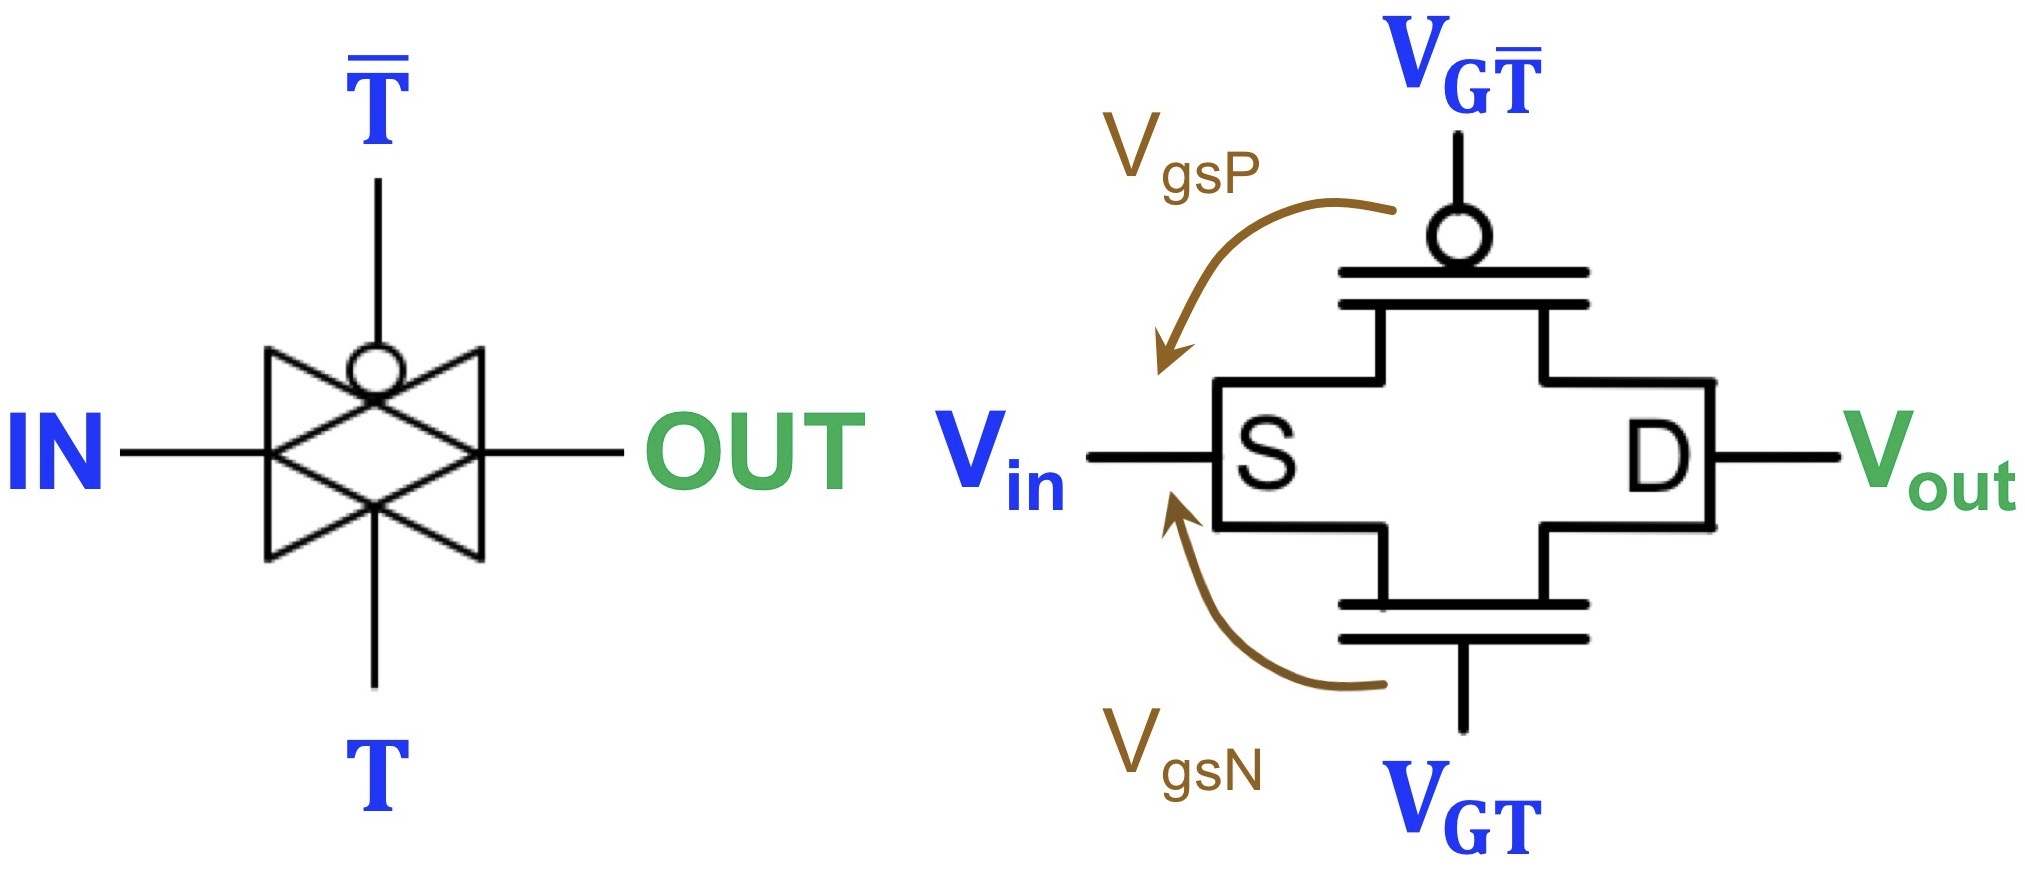
\includegraphics[height = 18mm]{images/tg.jpeg}
\end{center}
\begin{center}
    \small
    \begin{tabular}{c c|c|c}
        IN & T & Widerstand & OUT\\
        \hline
        0 & 0 & hochohm. & -\\
        0 & 1 & niederohm. & 0\\
        1 & 0 & hochohm. & -\\
        1 & 1 & niederohm. & 1\\
    \end{tabular}
\end{center}
TG sperrt wenn Widerstand hochohmig ist. ($\text{T}=0$)
\begin{center}
    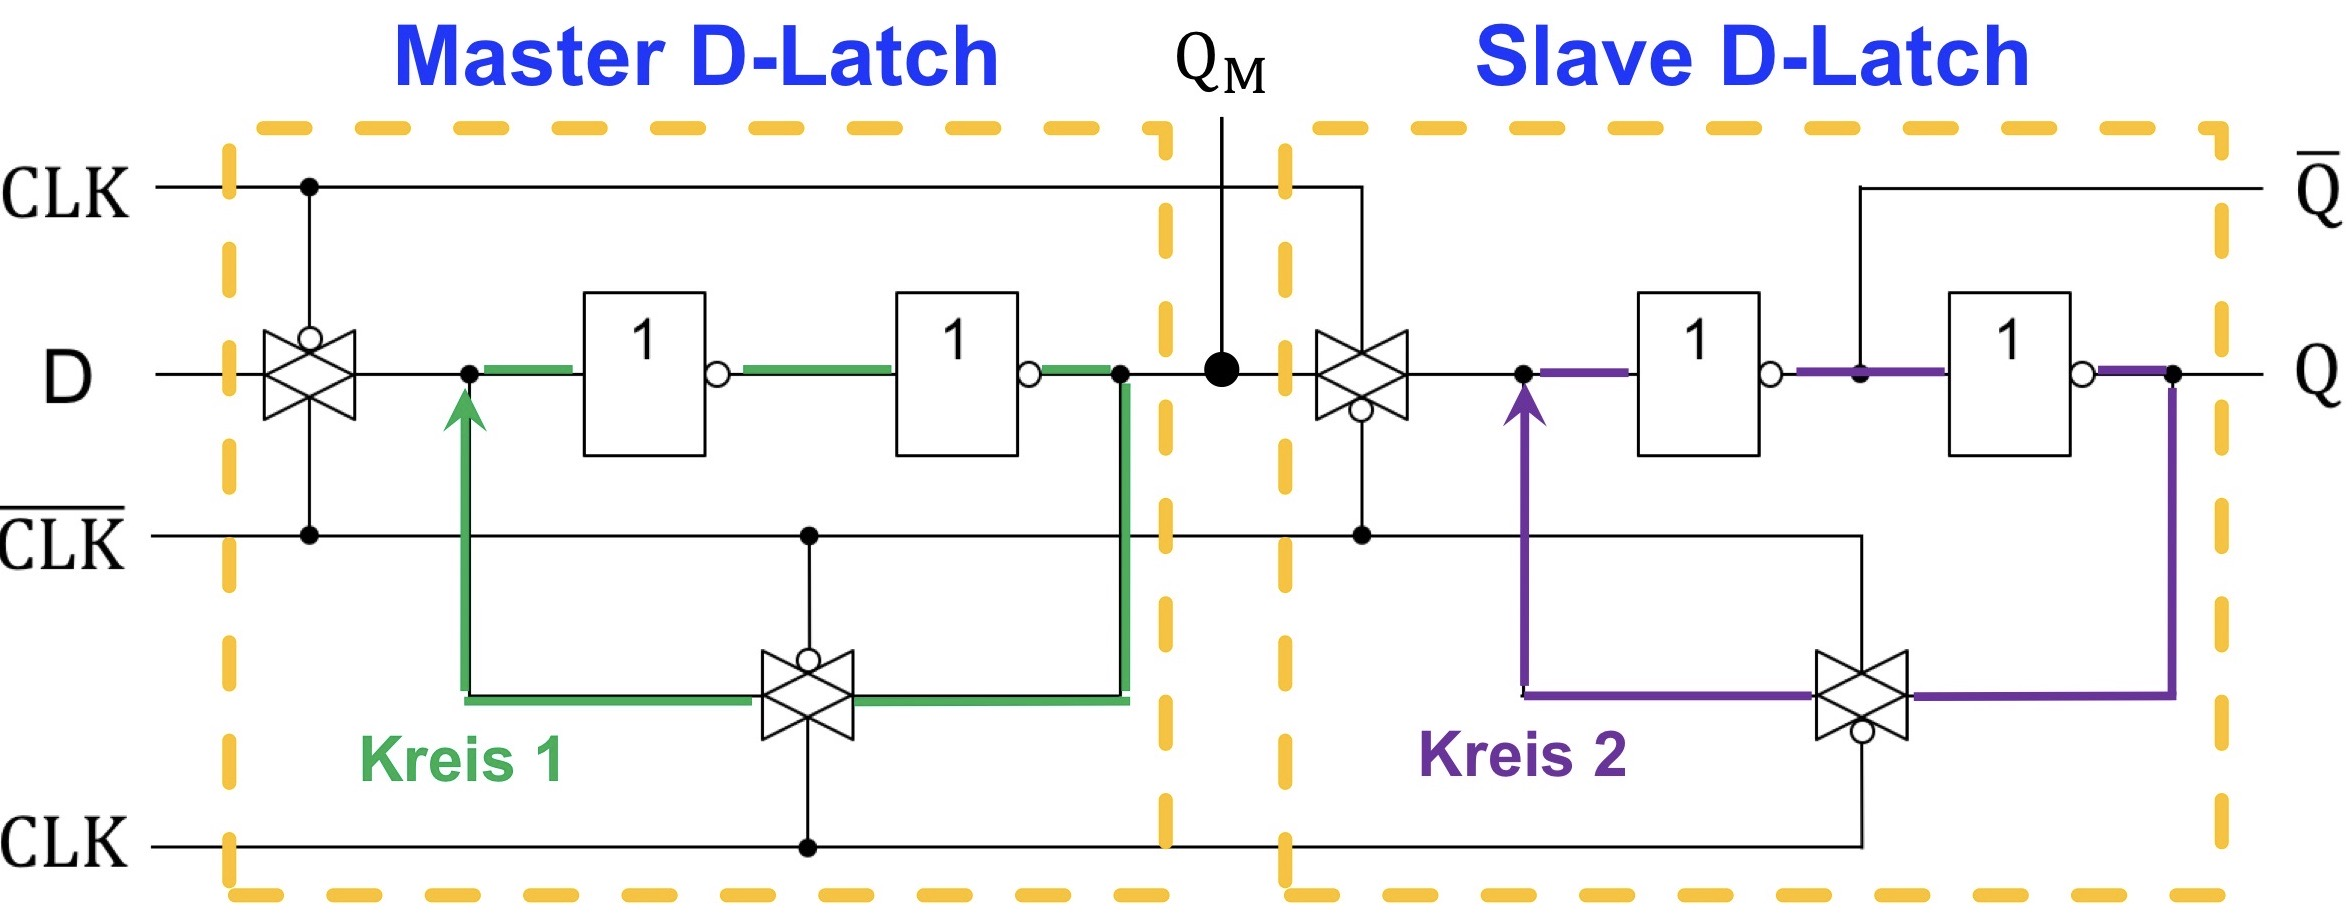
\includegraphics[width = 65mm]{images/d_ff_cmos.jpeg}
\end{center}
\begin{flushleft}
    \small
    \begin{tabular}{c l}
        CLK & \\
        0 & Input ins erste Latch übertragen\\
        1 & Latch verriegelt, Wert im Kreis gefangen
    \end{tabular}
\end{flushleft}
\begin{center}
    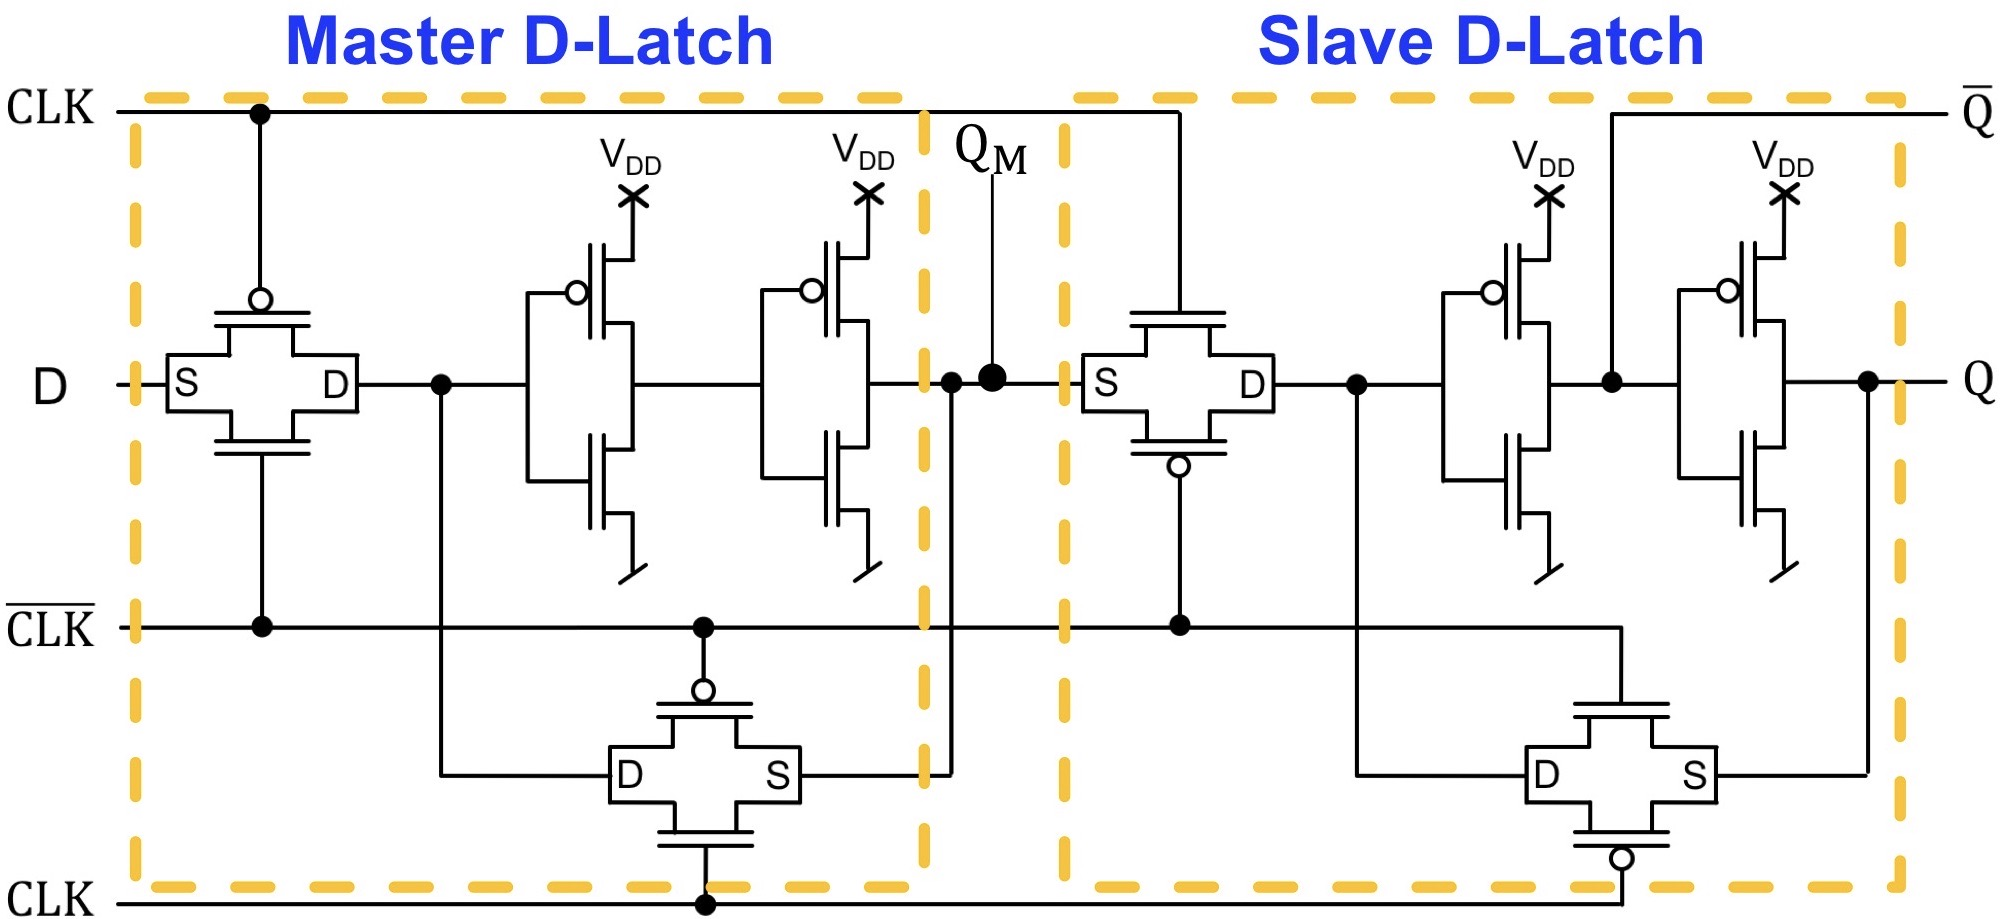
\includegraphics[width = 65mm]{images/d_ff_cmos_2.jpeg}
\end{center}
\subsubsection{D-FlipFlop $\Leftrightarrow$ JK-FlipFlop}
\begin{enumerate}
    \item JK-FF kann immer durch D-FF ersetzt werden.
    \begin{equation*}
        \text{D-FF:}\quad D_n = \left(J \land \overline{Q_n}\right) \lor \left(\overline{K} \land Q_n\right)\quad \text{:JK-FF}
    \end{equation*}
    \item Ein D-FF kann nur durch JK-FF ersetzt werden wenn:
    \begin{enumerate}
        \item Schaltung eine Rückkopplung enthält.
        \item Input D als $\left(F_1 \land \overline{Q_n}\right) \lor \left(F_2 \land Q_n\right)$ geschrieben werden kann.
    \end{enumerate}
\end{enumerate}
\paragraph{Gleichung für D-FF $\rightarrow$ JK-FF}
\begin{center}
    \begin{minipage}{0.65\linewidth}
        \begin{enumerate}
            \item Wahrheitstabelle mit Einängen und Rückkopplung.
            \item Wahrheitstabelle in \textcolor{pastelaqua}{$Q_n$} und \textcolor{pastelviolet}{$\overline{Q_n}$}.
            \item Separat Päckchen in \textcolor{pastelaqua}{$Q_n$} und \textcolor{pastelviolet}{$\overline{Q_n}$} machen.
            \item Päckchen mit OR verbinden. Ggf. \textcolor{pastelaqua}{$Q_n$} und \textcolor{pastelviolet}{$\overline{Q_n}$} ausklammern.
        \end{enumerate}
    \end{minipage}
    \hfill
    \begin{minipage}{0.3\linewidth}
        \begin{center}
            \begin{tikzpicture}
                \matrix (kv) [
                    matrix of nodes,
                    nodes in empty cells,
                    column sep=-\pgflinewidth, row sep=-\pgflinewidth,
                    nodes = {
                        rectangle,
                        draw = black,
                        text width = 1.3mm,
                        text height = 1.3mm,
                        align = center
                    }
                ]{
                \node[kvbinhead] {}; & \node[kvbinhead] {\tiny 00}; & \node[kvbinhead] {\tiny 01}; & \node[kvbinhead] {\tiny 11}; & \node[kvbinhead] {\tiny 10};\\
                \node[kvbinhead] {\tiny 00}; & & & &\\
                \node[kvbinhead] {\tiny 01}; & & & &\\
                \node[kvbinhead] {\tiny 11}; & & & &\\
                \node[kvbinhead] {\tiny 01}; & & & &\\
                };
    
                \node[] at ($(kv-1-1.north east) + (-1mm, -1mm)$) {\tiny $\text{Q}_\text{n}$A};
                \node[] at ($(kv-1-1.south west) + (1mm, 1mm)$) {\tiny BC};
                \draw[] ($(kv-1-1.north west) + (2mm, -2mm)$) -- (kv-1-1.south east);
                \fill[pastelviolet, opacity = 0.3] (kv-2-2.north west) rectangle (kv-5-3.south east);
                \fill[pastelaqua, opacity = 0.3] (kv-2-4.north west) rectangle (kv-5-5.south east);
            \end{tikzpicture}
        \end{center}
    \end{minipage}
\end{center}

\subsubsection{Asynchroner Set/Reset Input}
\begin{center}
    \begin{minipage}{0.55\linewidth}
        Können gespeicherte Zustände asynchron zu CLK überschreiben.
    \end{minipage}
    \hfill
    \begin{minipage}{0.4\linewidth}
        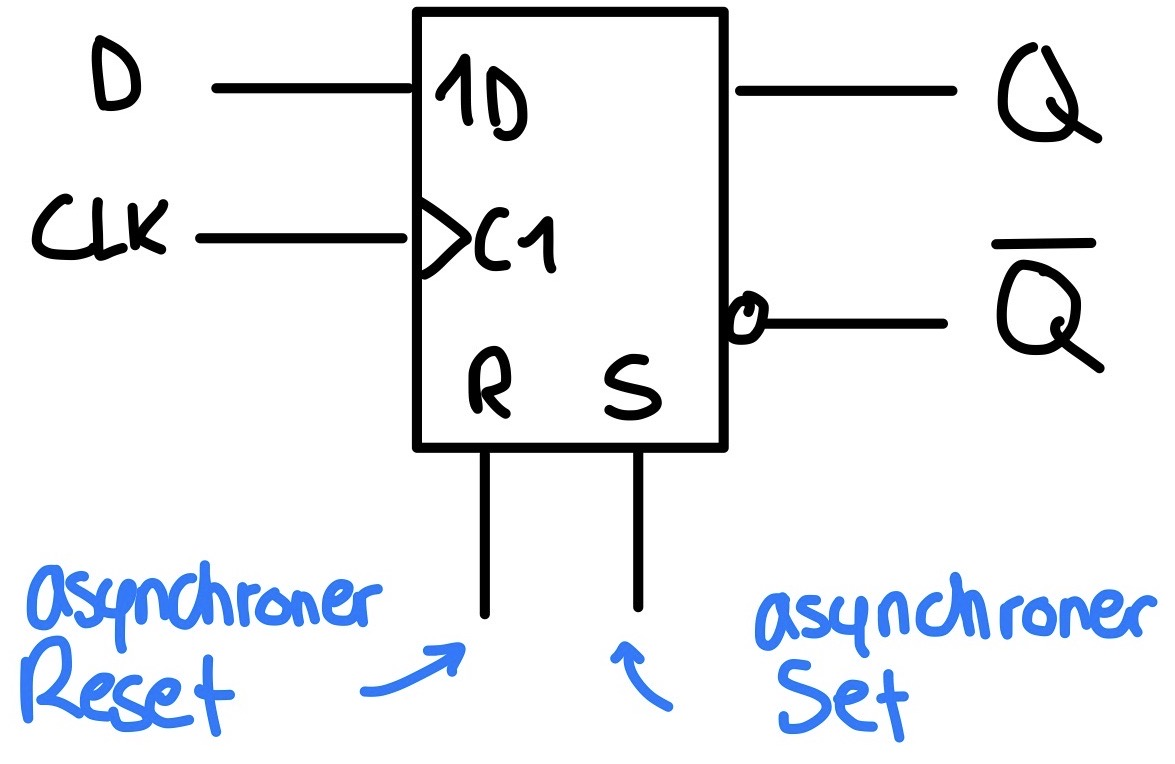
\includegraphics[width = 23mm]{images/async_sr.jpeg}
    \end{minipage}
\end{center}

\subsubsection{Verzögerungszeiten}
\begin{flushleft}
    \small
    \begin{tabular}{l l p{32mm}}
        $t_s$ & Setup-Zeit & Solange muss Signal \underline{vor} aktiver Taktflanke stabil anliegen.\\
        $t_h$ & Hold-Zeit & Solange muss Signal \underline{nach} aktiver Taktflanke stabil anliegen.\\
        $t_{pd}$ & Verzögerungszeit & Durchlaufzeit
    \end{tabular}
\end{flushleft}
\begin{equation*}
    T_{\text{min}} \geq t_{\text{pd}1} + t_{\text{pd,ks}} + t_{\text{s}2} \qquad f_{\text{max}} = \frac{1}{T_{\text{min}}}
\end{equation*}
$t_h$ kann bei der Berechnung von $f_{\text{max}}$ vernachlässigt werden.

\subsubsection{Zwischenspeicher-FF}
\begin{center}
    \begin{minipage}[c]{0.4\linewidth}
        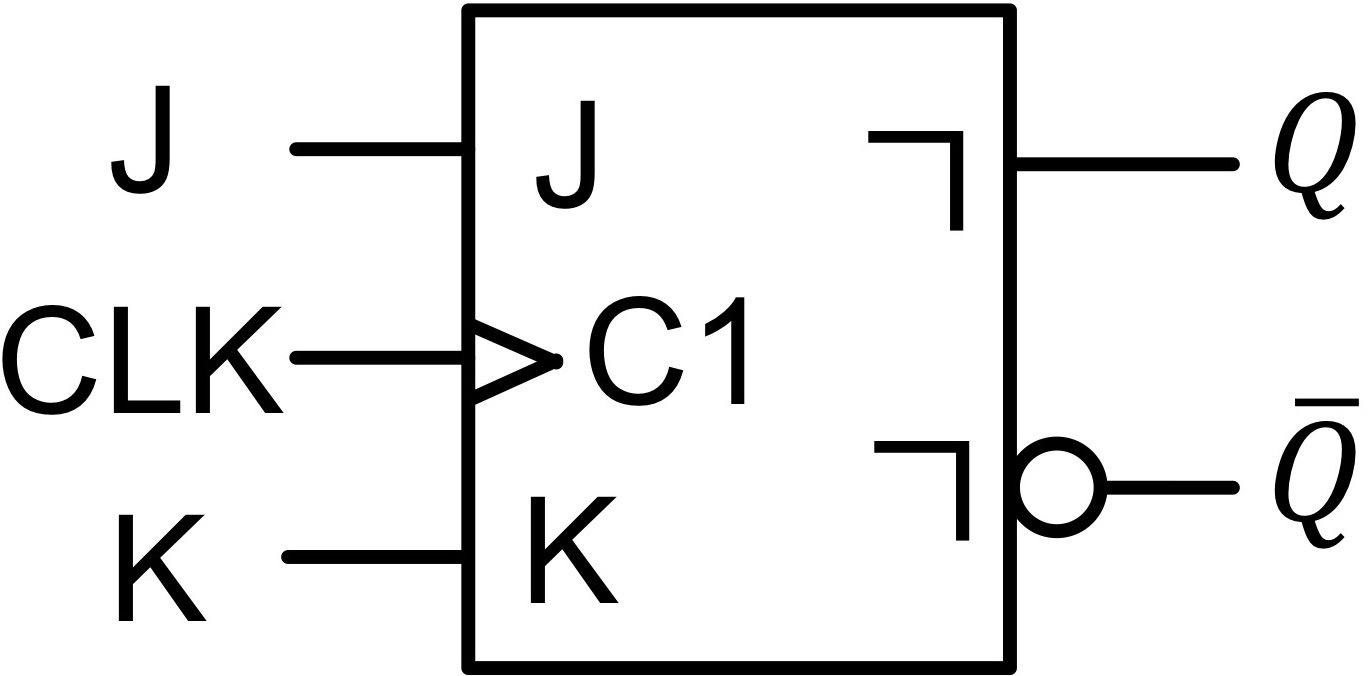
\includegraphics[width = 23mm]{images/zs_ff.jpeg}
    \end{minipage}
    \hfill
    \begin{minipage}[c]{0.55\linewidth}
        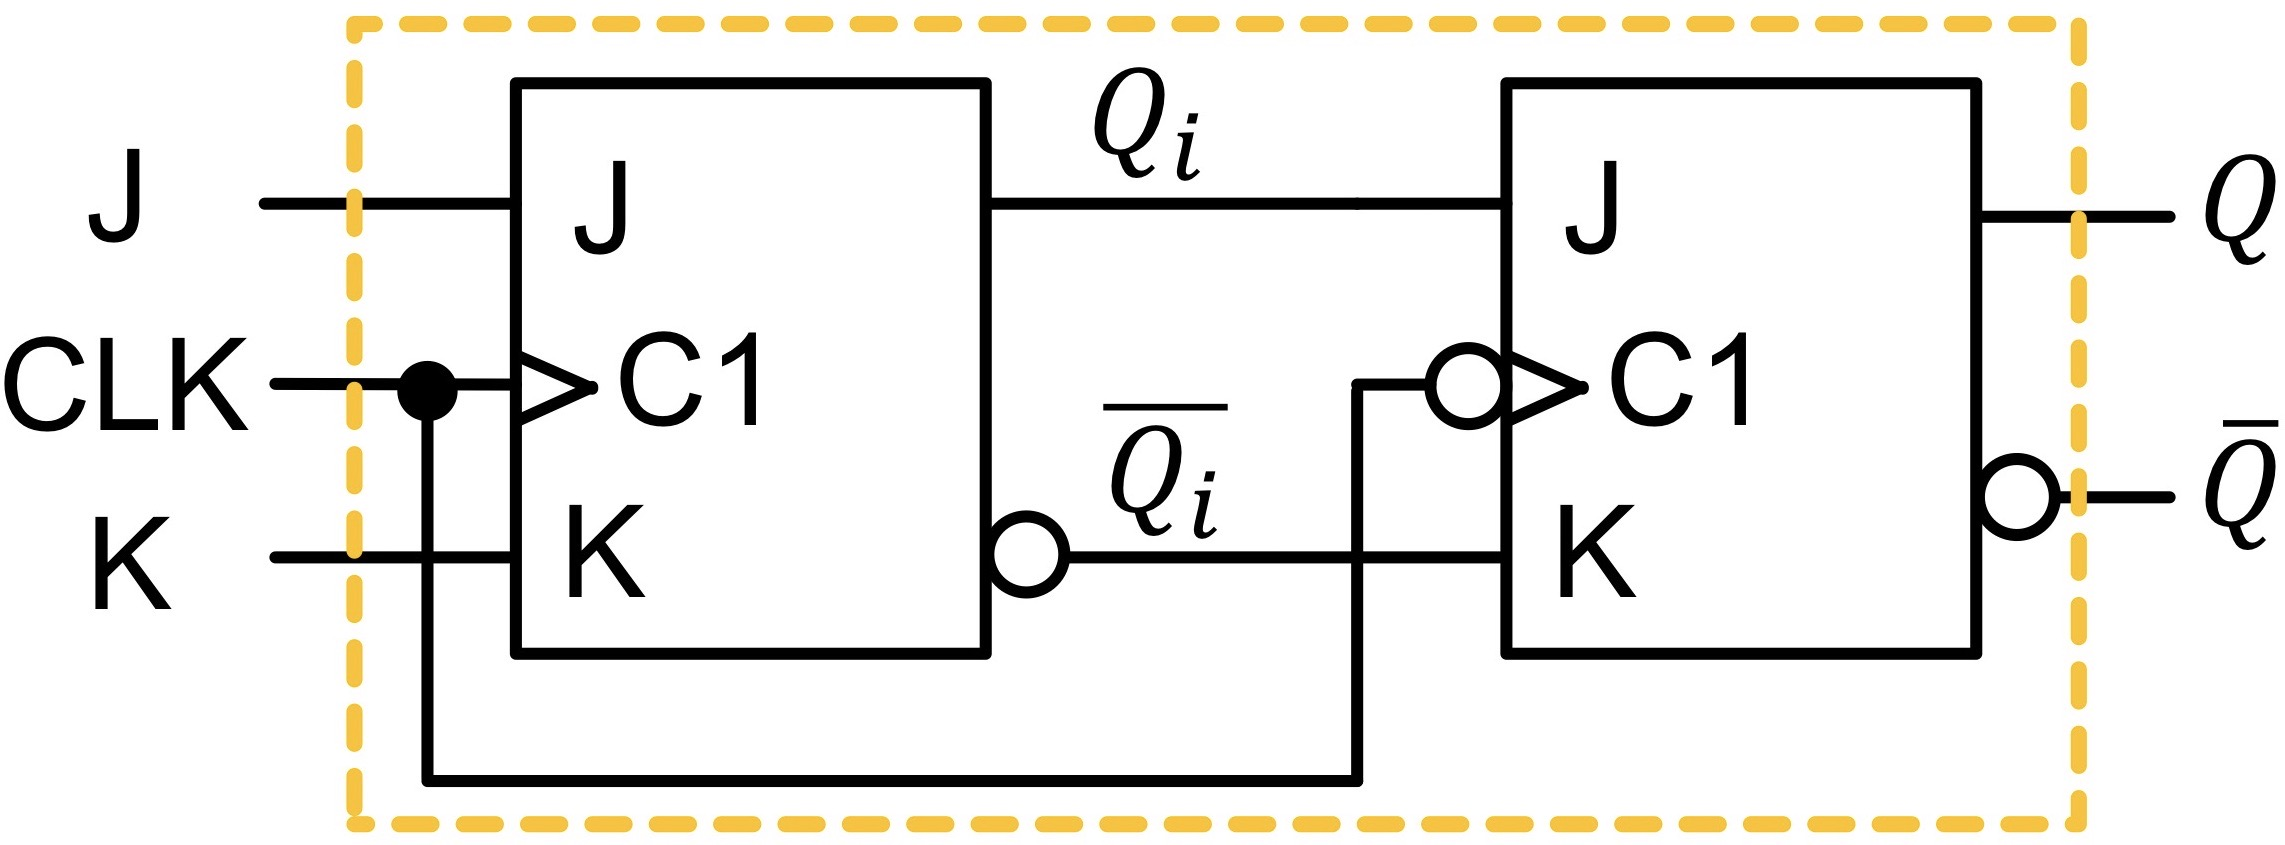
\includegraphics[width = 35mm]{images/zs_ff_cir.jpeg}
    \end{minipage}
\end{center}
FlipFlop, dass Input bei steigender Taktflanke übernimmt und bei der nächsten fallenden Taktflanke ausgibt. (oder umgekehrte Flanken)
\begin{flushleft}
    \begin{tabular}{c l}
        $\urcorner$ & Ausgabe bei fallender Flanke\\
        $\lrcorner$ & Ausgabe bei steigender Flanke\\
    \end{tabular}
\end{flushleft}

\subsubsection{Frequenzteiler und Zähler}
\begin{center}
    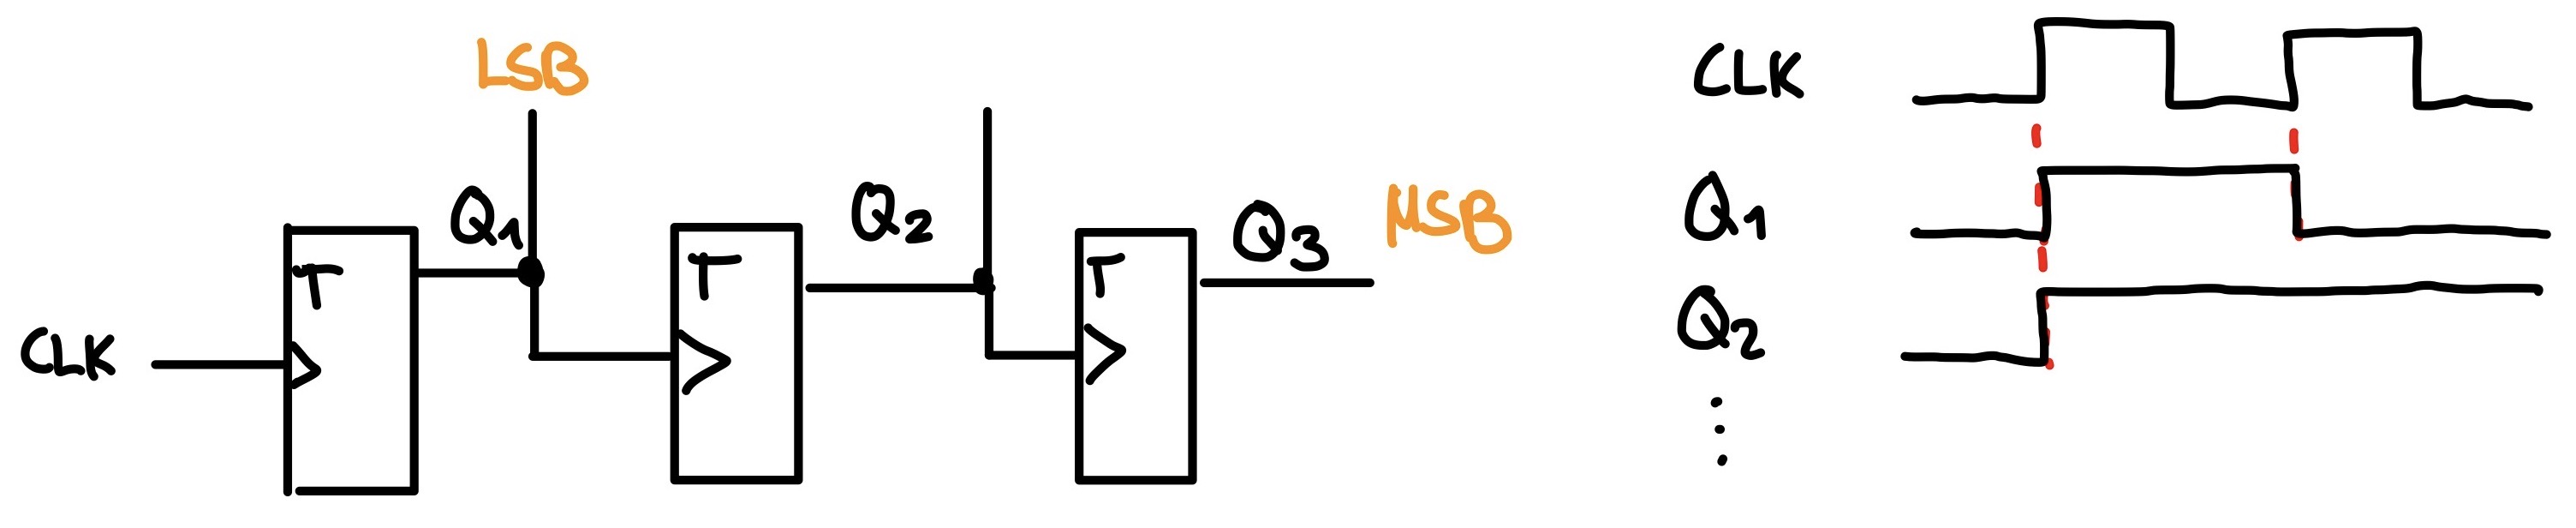
\includegraphics[width = 65mm]{images/counter.jpeg}
\end{center}
Kaskadeuren von T-Flipflops führt zu einer Frequenzreduktion von CLK um Faktor 2.\\
Kann als Bitzähler verwendet werden (ohne CLK). MSB ist längste Frequenz. $n_{T,ff} \rightarrow 0\dots (2^n -1)$